\documentclass{article}
\usepackage[margin=1in]{geometry}
\usepackage{graphicx}
\usepackage{xcolor}
\usepackage{float}
\usepackage{amsmath}
\usepackage{cite}
\usepackage{hyperref}
\usepackage{indentfirst}
\graphicspath{{..} {./images}}

\definecolor{navy-blue}{rgb}{0.22,0.38,0.71}

\renewcommand{\contentsname}{\vspace*{-2\baselineskip}}

\hypersetup{
	colorlinks,
	linkcolor=black,
	urlcolor=blue,
	citecolor=black
}
  		
\begin{document}
\begin{titlepage}
	\centering
	{\huge Lab 5 - Digital Modulation: Symbol Synchronization}\\[0.25 in]
	
\includegraphics[width=0.6\textwidth]{ua_logo.png}\\[0.25 in]
	{\large \textbf{ECE 531 - Software Defined Radio\\[0.25 in]
	April 7, 2025\\[0.25 in]}}
	{\large Owen Sowatzke, osowatzke@arizona.edu\\[0.05 in]
	Department of Electrical \& Computer Engineering\\[0.05 in]
	University of Arizona, Tucson, AZ 85721\\[0.5 in]}
	\hypersetup{linkcolor=navy-blue}
	\noindent\hrulefill
	\tableofcontents
	\noindent\hrulefill
\end{titlepage}

% \setlength{\parindent}{0pt}

\section{Introduction}
%Introduction to the laboratory experiment, including a brief description of the objectives and goals.

In this lab, we focus on pulse shaping, matched filtering, timing errors, and symbol timing synchronization. We start by analyzing pulse shaping and matched filtering. Next, we discuss timing errors and examine their impact on data captured with our PlutoSDR. Then, we learn how to perform symbol timing compensation using the Zero Crossing, Garnder, and M\"{u}ller and Mueller methods. We specifically implement one of the these timing compensation methods in MATLAB. Then, for a slowly-varying timing offset, we measure the error vector magnitude (EVM) before and after timing compensation. We also introduce a phase offset and see how it impacts our results. Next, we examine the data rates of our timing compensation logic and understand how our logic can be integrated into the receiver. Similar to our previous analysis, we measure the EVM with no timing offsets, a fixed timing offset, and a fixed phase offset. Finally, we perform timing compensation on PlutoSDR data and compare the resulting EVMs to the EVMs we measured in simulation.  The lab report that follows is divided into two primary sections. One presents the procedures for each of our experiments and the other covers the results.  

%Introduction to the laboratory experiment, including a brief description of the objectives and goals.
% In this report, we will examine time offset errors and their impact on sampling and recovery in digital communications systems. We will implement three timing compensation methods: Zero crossing, Gardner, and Muller and Mueller method. To evaluate signal quality with these methods, we will derive EVM measurements before and after time correction. 

% Next, we will assess the impact of phase offsets on reference constellations which may cause EVM degradation. Finally, we will determine the ideal recovery block placement for time and phase alignment for improved performance across different SNR conditions.

\section{Procedure}
% Detailed explanation of the laboratory experiment, including the design, implementation, and testing of the system.

In this section, we review the procedure for each of our experiments. We start by analyzing pulse shaping and matched filtering. Next, we examine the impacts of timing errors. Then, we learn how to perform symbol timing compensation and analyze how timing compensation can be integrated into the overall system. Finally, we perform symbol timing compensation on data collected with the PlutoSDR.

\subsection{Pulse Shaping and Matched Filtering}

In this experiment, we analyze the effects of pulse shaping and matched filtering. Pulse shaping and match filtering together serve 3 purposes: limiting signal bandwidth, maximizing SNR, and minimizing ISI. In this experiment, we use an SRRC filter which is defined as follows:

\begin{equation}
	h(t) = \begin{cases}
		\frac{1}{\sqrt{T_s}}\left(1 - \beta + 4\frac{\beta}{\pi}\right), & t = 0 \\
		\frac{\beta}{\sqrt{2T_s}}\left[\left(1 + \frac{2}{\pi}\right)\sin\left(\frac{\pi}{4\beta}\right)+ \left(1-\frac{2}{\pi}\right)\cos\left(\frac{\pi}{4\beta}\right)\right], & t = \pm\frac{T_s}{4\beta} \\
		\frac{1}{\sqrt{T_s}}\frac{\sin\left[\pi\frac{t}{T_s}(1-\beta)\right]+4\beta\frac{t}{T_s}\cos\left[\pi\frac{t}{T_s}(1+\beta)\right]}{\pi\frac{t}{T_s}\left[1 - \left(4\beta\frac{t}{T_s}\right)^2\right]}, & \text{otherwise}
	\end{cases}
	\label{eq::srrc_filter}
\end{equation}

\noindent In the above formula, $T_s$ is the symbol period and $\beta \in [0,1]$ is the roll-off factor. The SRRC filter belongs to a subset of filters called Nyquist filters, which have zero ISI when sampled at the correct instances. As part of our work in this section, we explain the differences between type I and type II Nyquist filters. Then, we generate frequency response plots for SRRC filters with $\beta \in [0, 0.1, 0.25, 0.5, 0.1]$ and discuss how the roll-off factor affects spectral efficiency and filter complexity. Next, we generate transmit and receive plots following the template included in the lab description and on page 196 of the textbook. Using these plots, we analyze how the roll-off factor affects timing recovery performance.

\subsection{Timing Error}

In this experiment, we analyze the impact of timing errors (when the transmitter and receiver are not sampling at the same time instances). For this experiment, we transmit QPSK symbols on the Pluto SDR loopback cable and examine the resulting constellations. We then highlight the effects of timing offsets and explain any rotation we observe in the constellation.

\subsection{Symbol Timing Compensation}

In this experiment, we learn how to perform symbol timing compensation. The algorithm we implement specifically follows the structure shown in Figure \ref{fig::timing_recovery_block_diagram}.

\begin{figure}[H]
	\centerline{\fbox{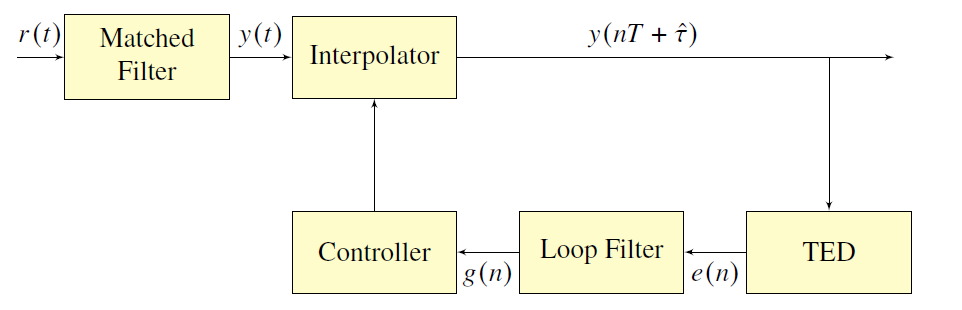
\includegraphics[width=0.7\textwidth]{timing_recovery_block_diagram.png}}}
	\caption{Structure of Timing Recovery PLL}
	\label{fig::timing_recovery_block_diagram}
\end{figure}

\noindent In the above figure, the interpolator applies a fractional delay. The timing error detector (TED) measures the time offsets. The loop filter stabilizes error correction, and the interpolator controller manages the interpolation process.

\subsubsection{Timing Error Detector}
For the timing error detector, three common algorithms are the zero-crossing (ZC) method, the Gardner method, and the M\"{u}ller and Mueller method. For the experiments in this lab, we use the zero-crossing method which operates as follows:

\begin{align}
	e(k) = &\text{Re}(x((k-1/2)T_s + \tau))\left[\text{sgn}\{\text{Re}(x((k-1)T_s+\tau))\} - \text{sgn}\{\text{Re}(x(kT_s+\tau))\}\right] + \\
	&\text{Im}(x((k-1/2)T_s + \tau))\left[\text{sgn}\{\text{Im}(x((k-1)T_s+\tau))\} - \text{sgn}\{\text{Im}(x(kT_s+\tau))\}\right]
\end{align}

\noindent To ensure only one update per symbol, the timing error detector only outputs an error when it receives a strobe. Otherwise, it outputs a zero.

\subsubsection{Loop Filter}
The timing error detector output is then fed into the loop filter, which produces a stable signal for the controller. The loop filter is a proportional integral (PI) filter and is defined as follows:

\begin{equation}
	y(n) = G_1x(n) + G_2\sum_{k=0}^{n}{x(k)}
\end{equation}

\noindent In the above equation, $G_1$ and $G2$ are constants defined as follows:

\begin{align}
	G_1 = \frac{-4\zeta\theta}{G_DN\Delta} && G_2 = \frac{4\theta^2}{G_DN\Delta}
\end{align}

\noindent and $\theta$ and $\Delta$ are further defined follows:

\begin{align}
	\theta = \frac{B_{\text{Loop}}}{M(\zeta + 0.25/\zeta)} && \Delta = 1 + 2\zeta\theta + \theta^2
\end{align}

\noindent In the above equations:

\begin{itemize}
	\item $B_{\text{Loop}}$ is the normalized loop bandwidth
	\item $\zeta$ is the damping factor
	\item $N$ is the samples per symbol
	\item $G_D$ is the detector gain (scaling factor for correction)
\end{itemize}

\subsubsection{Interpolation Controller}

The loop filter output is then fed into an interpolation controller, which computes a fractional delay and a strobe which indicates when the delay should be applied. The strobes occur on average once per symbol. The counter decrement value can be computed with the loop filter output $v(n)$ as follows:

\begin{equation}
	W(n) = v(n) + \frac{1}{N}
\end{equation}

\noindent Using the decrement, the counter is updated as follows:

\begin{equation}
	c(n + 1) = (c(n) - W(n))\ \text{mod}\ 1
\end{equation}

\noindent Strobes occur whenever the counter wraps.

\begin{equation}
	\text{Strobe} = \begin{cases}
		\text{True}, & \text{if}\ c(n) < W(n)\\
		\text{False}, & \text{otherwise}
	\end{cases}
\end{equation}

\noindent Finally, on each strobe, we update the factional delay parameter as follows:

\begin{equation}
	\mu(k) = \frac{c(n)}{W(n)}
\end{equation}

\subsubsection{Interpolator}

The interpolator applies fractional delays to the input signal. It specifically using a piecewise polynomial filter (PPF) which approximates the required delays. The filter output is given by

\begin{equation}
	x(kT_s + \mu(k)T_s) = \sum_{n=-2}^{1}{h(n)x((k-n)T_s)}
\end{equation}

\noindent And the filter taps $h(n)$ are given as

\begin{equation}
\begin{split}
	h = [&\alpha\mu(k)(\mu(k) - 1), \\
	&-\alpha\mu(k)^2 - (1-\alpha)\mu(k) + 1,\\
	&-\alpha\mu(k)^2 + (1+\alpha)\mu(k),\\
	&\alpha\mu(k)(\mu(k) - 1)]
\end{split}
\end{equation}

\subsubsection{Implementation}

Following the flowchart shown in Figure \ref{fig::timing_recovery_block_diagram}, we implement timing compensation in MATLAB and compare the behavior of our implementation to MATLAB's \texttt{comm.SymbolSychronizer} object. Next, we use our custom implementation to perform timing compensation on an input with a slowly-changing timing offset. We perform error vector magnitude (EVM) measurements of the signal before and after timing compensation at different SNR levels using MATLAB's \texttt{comm.EVM} object. Then, we add a fixed phase offset of $\pi/8$ radians and repeat the EVM measurements. We compare the EVM before and after adding the phase offset and explain how it affects timing recovery performance.

\subsection{Adding Pieces Together}
\label{section::sim_procedure}

In this section, we investigate how the timing compensation logic can be integrated into the overall system.  Figure \ref{fig::timing_recovery_integration} shows the data flow from transmitter to receiver.

\begin{figure}[H]
	\centerline{\fbox{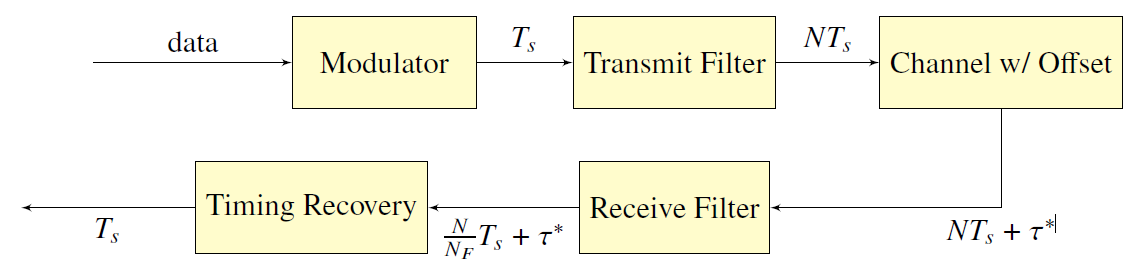
\includegraphics[width=0.7\textwidth]{timing_recovery_integration.png}}}
	\caption{Integration of Timing Recovery Logic into Overall System}
	\label{fig::timing_recovery_integration}
\end{figure}

\noindent The modulator generates symbols at the symbol rate, and the transmit filter increases the sample rate by a factor of $N$. The data then flows through the channel which applies a delay and noise. Next, the data passes through the receive filter, which downsamples the data by a factor of $N_F$ where $N_F \leq N$. Finally, the timing recovery circuit removes the timing offset and generates symbols at the symbol rate.

	In this experiment, we expand on the timing recovery block shown in Figure \ref{fig::timing_recovery_integration}. We detail each of its subblocks and discuss the number of samples per symbol that each of them process. Finally, we use the timing recovery block to perform timing compensation under a variety of conditions:
	
	\begin{itemize}
		\item No offsets (ideal baseline case)
		\item A fixed timing offset of $0.25T_s$
		\item A fixed phase offset of $\pi/4$ radians.
	\end{itemize}	
	
	\noindent For each case we measure the resulting EVM over a range of SNR values.
	
\subsection{Testing on Hardware}

In this experiment, we performing timing correction on data captured with the PlutoSDR. We specifically transmit a DBPSK or QPSK reference signal in a loopback configuration and perform timing correction on the received signal. Using our collected data we compute the error vector magnitude (EVM) before and after timing correction. We compare these results to the simulation results captured in Section \ref{section::sim_procedure}. Using the comparison results, we highlight any differences in performance. Then, we discuss challenges in the hardware implementation and any algorithm modifications that we needed to make when moving from simulation to hardware.

\section{Results}
% Results and discussion of the laboratory experiment, including captured outputs, observations, and responses to laboratory questions.

In this section, we review the results for each of our experiments. We start by analyzing pulse shaping and matched filtering. Next, we examine the impacts of timing errors. Then, we learn how to perform symbol timing compensation and analyze how timing compensation can be integrated into the overall system. Finally, we perform symbol timing compensation on data collected with the PlutoSDR.

\subsection{Pulse Shaping and Matched Filtering}

In this experiment, we study pulse shaping and matched filtering. We start by examining the difference between type I and type II Nyquist filters. Then, we examine how the roll-off factor ($\beta$) effects spectral efficiency and filter complexity. Finally, we determine how different roll-off factors affect timing recovery performance.

Type I Nyquist filters are defined by a rectangular pulse in the frequency domain and a sinc pulse in the time domain. The sinc pulse has zero crossings at $nT$, which produces zero ISI. Because Type I Nyquist filters are a rectangular pulse in the frequency-domain, they have the minimum bandwidth and maximize spectral efficiency. However, there are a couple problems with type I Nyquist filters. First, they are infinite in time. Second, accurate sampling is required. Small timing errors can result in large ISI because the impulse response of a sinc filter decays with $1/t$, which does not converge.

Type II Nyquist filters also have zero crossing at $nT$. However, they have a bandwidth larger than the minimum bandwidth, which allows them to achieve lower ISI sensitivity than type I Nyquist filters. The raised cosine filter is an example of a type II Nyquist filter. Its impulse responses decays with $1/t^3$, which quickly converges in the presence of timing errors.

Next, we compare the frequency response of the SRRC filters for $\beta \in [0,0.1,0.25,0.5,1]$. These frequency responses for these filters are captured in Figures \ref{fig::srrc_freq_response_beta_0} - \ref{fig::srrc_freq_response_beta_1}.

\begin{figure}[H]
	\centerline{\fbox{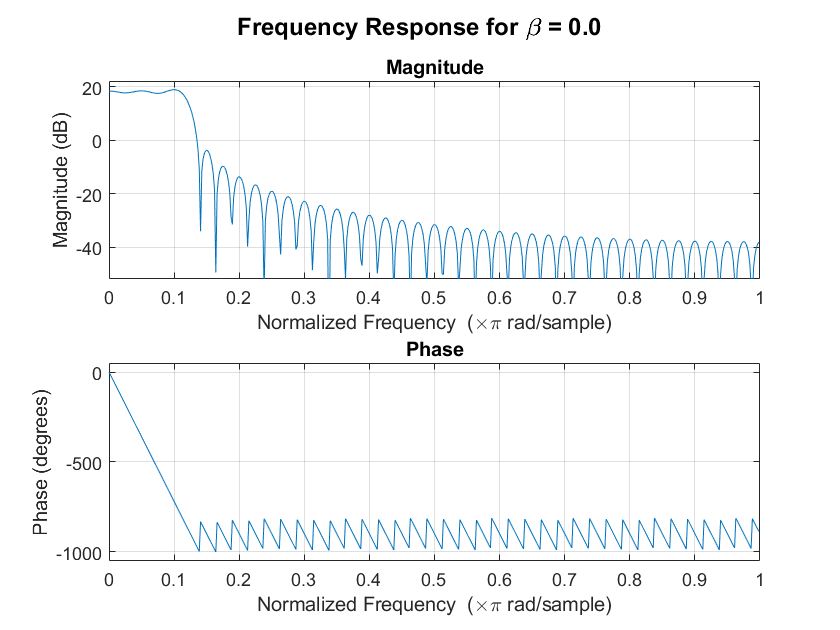
\includegraphics[width=0.5\textwidth]{srrc_freq_response_beta_0.png}}}
	\caption{SRRC Filter Frequency Response with $\beta=0$}
	\label{fig::srrc_freq_response_beta_0}
\end{figure}

\begin{figure}[H]
	\centerline{\fbox{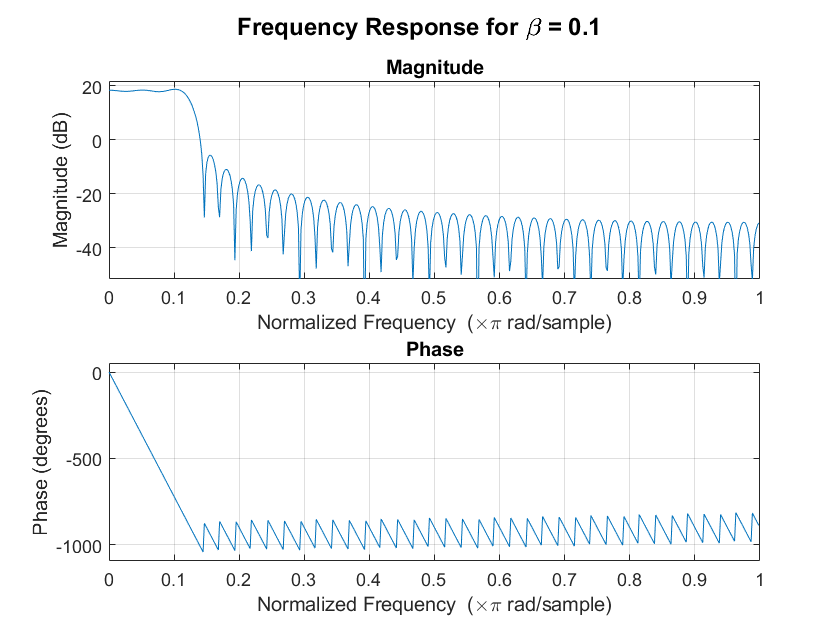
\includegraphics[width=0.5\textwidth]{srrc_freq_response_beta_0_1.png}}}
	\caption{SRRC Filter Frequency Response with $\beta=0.1$}
	\label{fig::srrc_freq_response_beta_0_1}
\end{figure}

\begin{figure}[H]
	\centerline{\fbox{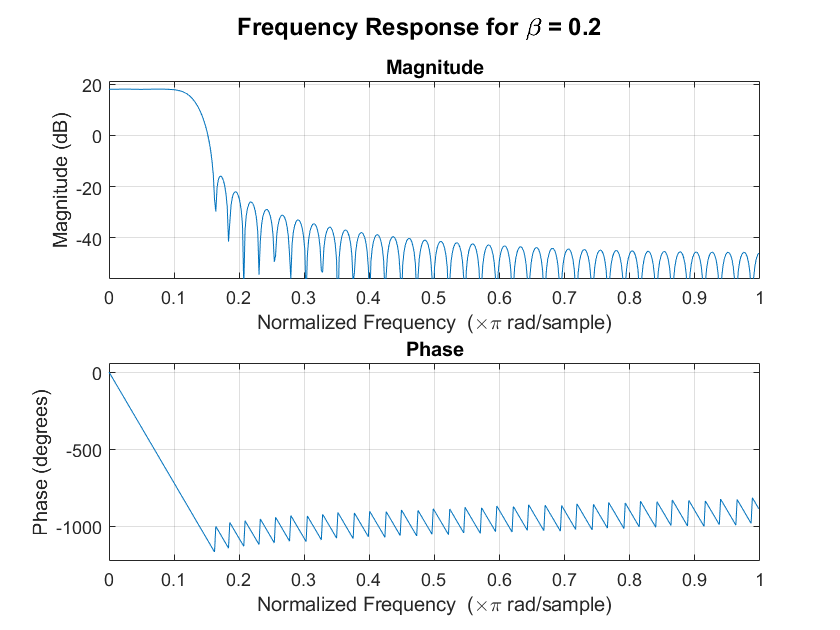
\includegraphics[width=0.5\textwidth]{srrc_freq_response_beta_0_2.png}}}
	\caption{SRRC Filter Frequency Response with $\beta=0.2$}
	\label{fig::srrc_freq_response_beta_0_2}
\end{figure}

\begin{figure}[H]
	\centerline{\fbox{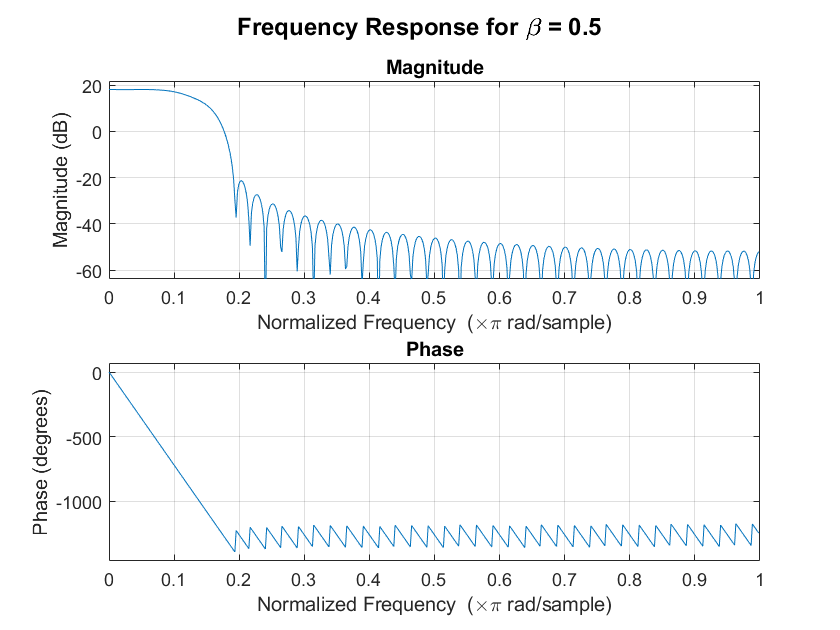
\includegraphics[width=0.5\textwidth]{srrc_freq_response_beta_0_5.png}}}
	\caption{SRRC Filter Frequency Response with $\beta=0.5$}
	\label{fig::srrc_freq_response_beta_0_5}
\end{figure}

\begin{figure}[H]
	\centerline{\fbox{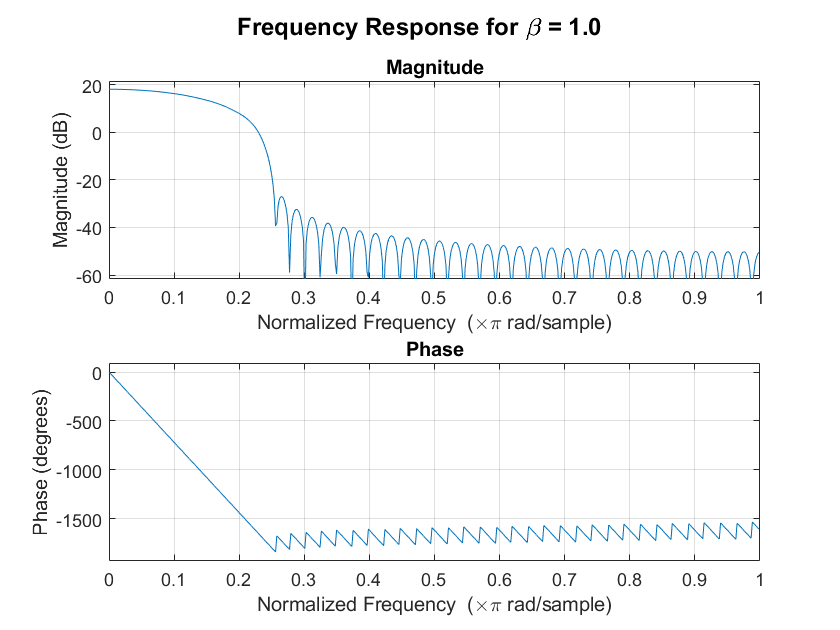
\includegraphics[width=0.5\textwidth]{srrc_freq_response_beta_1.png}}}
	\caption{SRRC Filter Frequency Response with $\beta=1$}
	\label{fig::srrc_freq_response_beta_1}
\end{figure}

\noindent Examining the frequency response of each of the filters, we see that the spectral efficiency is maximized for small values of the rolloff factor, $\beta$. However, the sharp filter transitions required for small $\beta$ increase the complexity of the filter. We can confirm this by the filter's impulse response for $\beta=0$ and $\beta=1$.

\begin{figure}[H]
	\centerline{\fbox{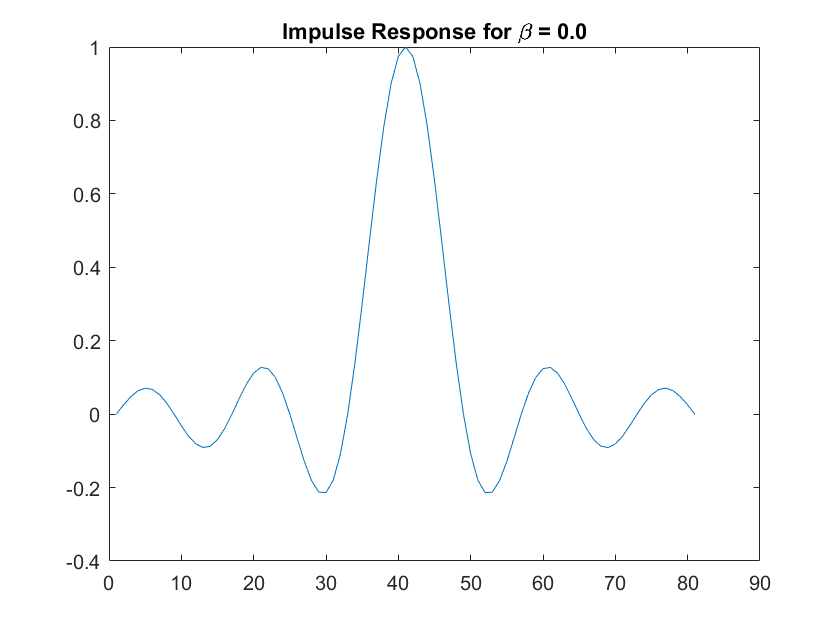
\includegraphics[width=0.5\textwidth]{srrc_impulse_response_beta_0.png}}}
	\caption{SRRC Filter Impulse Response with $\beta=0$}
	\label{fig::srrc_impulse_response_beta_0}
\end{figure}

\begin{figure}[H]
	\centerline{\fbox{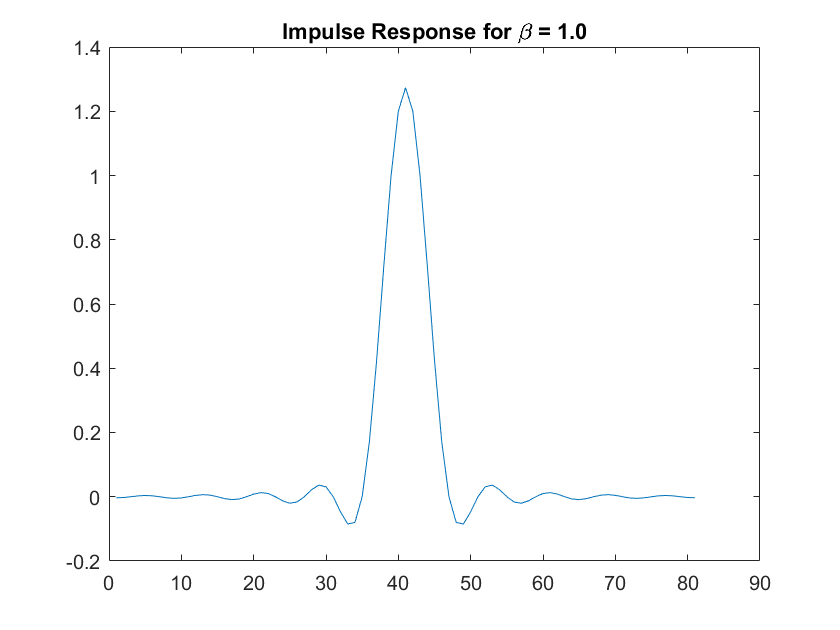
\includegraphics[width=0.5\textwidth]{srrc_impulse_response_beta_1.png}}}
	\caption{SRRC Filter Impulse Response with $\beta=1$}
	\label{fig::srrc_impulse_response_beta_1}
\end{figure}

\noindent Comparing the two impulses responses, we see that the impulse response with $\beta=1$ converges much faster than the impulse response with $\beta=0$. This allows us to truncate the impulse response sooner, which in turn reduces the filter length and complexity.

Finally, we examine how different rolloff factors affect timing recovering performance. To do this we analyze the received filter output for $\beta \in [0.1, 0.5, 0.9]$. Our results are captured in Figures \ref{fig::timing_recovery_beta_0_1} - \ref{fig::timing_recovery_beta_0_9}.

\begin{figure}[H]
	\centerline{\fbox{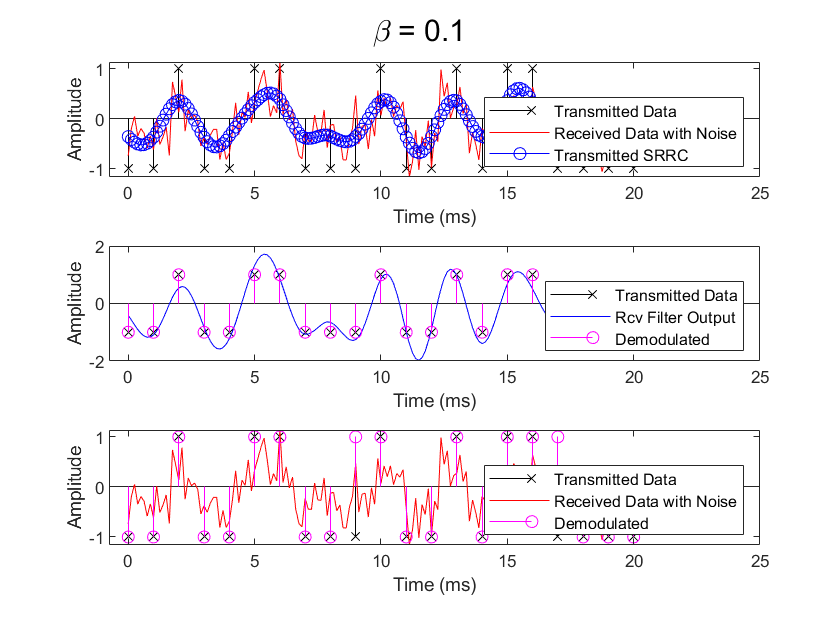
\includegraphics[width=0.5\textwidth]{timing_recovery_beta_0_1.png}}}
	\caption{Timing Recovery with $\beta=0.1$}
	\label{fig::timing_recovery_beta_0_1}
\end{figure}

\begin{figure}[H]
	\centerline{\fbox{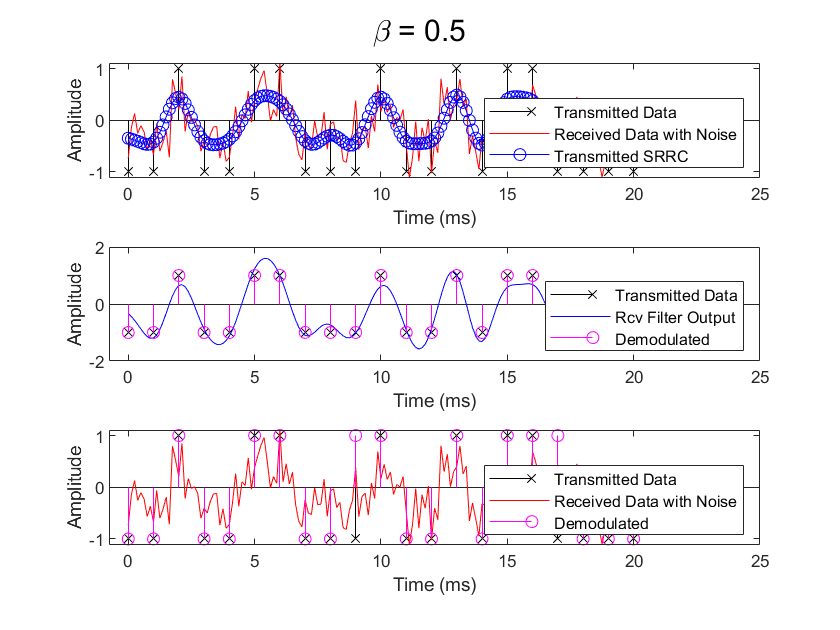
\includegraphics[width=0.5\textwidth]{timing_recovery_beta_0_5.png}}}
	\caption{Timing Recovery with $\beta=0.5$}
	\label{fig::timing_recovery_beta_0_5}
\end{figure}

\begin{figure}[H]
	\centerline{\fbox{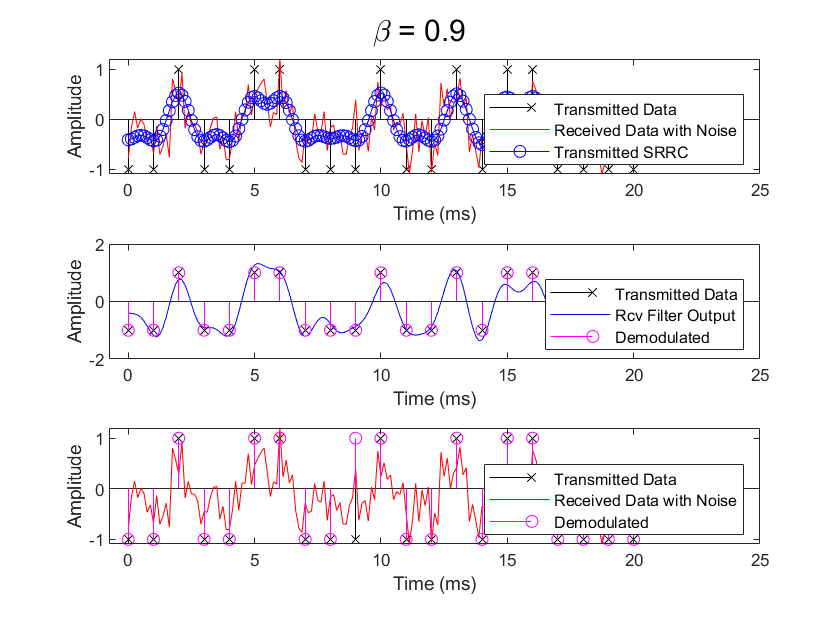
\includegraphics[width=0.5\textwidth]{timing_recovery_beta_0_9.png}}}
	\caption{Timing Recovery with $\beta=0.9$}
	\label{fig::timing_recovery_beta_0_9}
\end{figure}

\noindent The received filter outputs (shown in solid blue) allow us to visualize the effect of various timing offsets. For large values of $\beta$, the receive filter output creates better-defined symbols transitions, which in turn improve the performance of the timing recovery algorithm. Additionally, large values of $\beta$ results in less symbol overshoot, which reduces the impact of small timing errors.

\subsection{Timing Error}

In this section, we examine the effect of timing error. We specifically capture a QPSK constellation with the PlutoSDR. Our captured constellation is shown in Figure \ref{fig::pluto_constellation_raw} and contains both phase and timing offsets.

\begin{figure}[H]
	\centerline{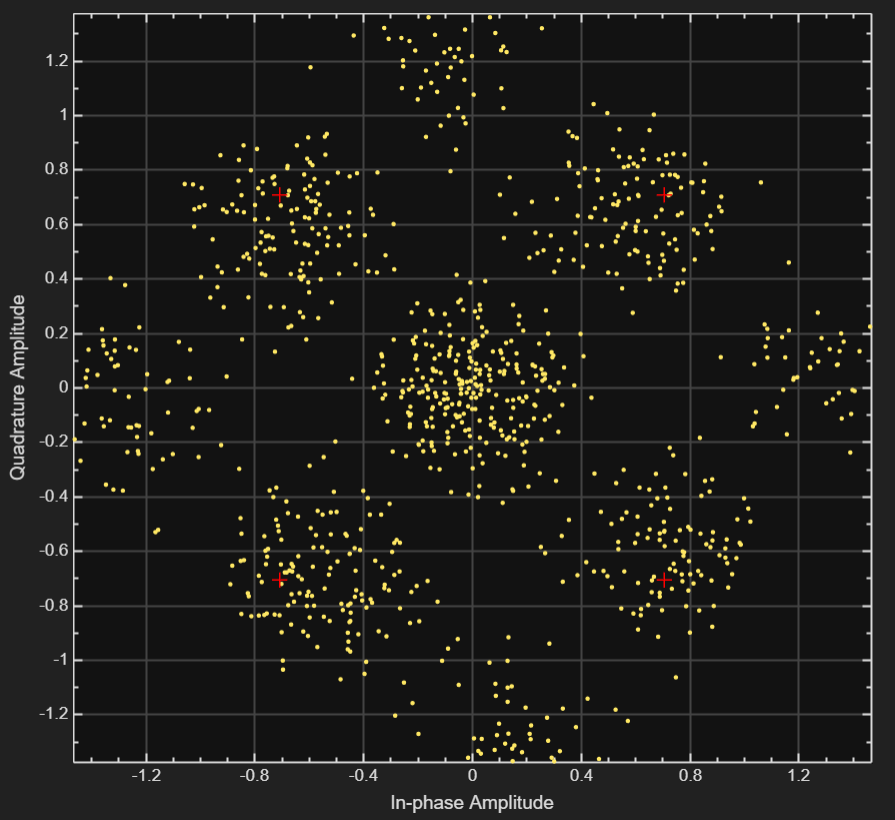
\includegraphics[width=0.5\textwidth]{pluto_constellation_raw.png}}
	\caption{QPSK Constellation Captured with Pluto SDR}
	\label{fig::pluto_constellation_raw}
\end{figure}

\noindent We also leverage code from \texttt{plutoLoopback.m} to sweep timing offsets. If we sweep the timing offsets, we can perform a manual timing compensation. With the best timing compensation, we get the constellation shown in Figure \ref{fig::pluto_constellation_best}.

\begin{figure}[H]
	\centerline{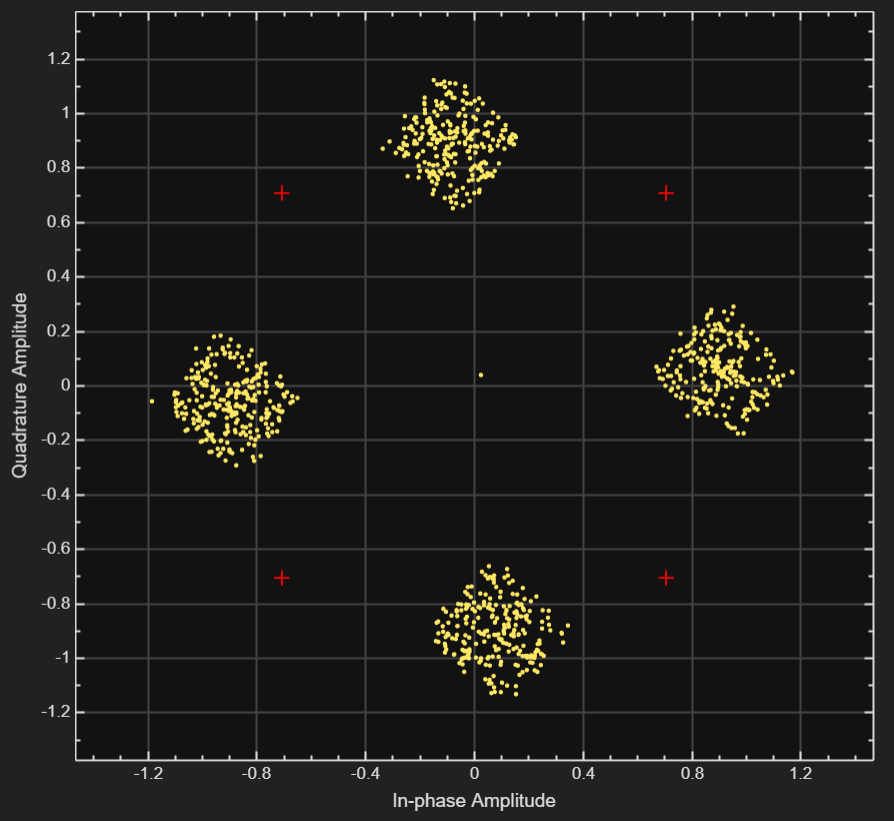
\includegraphics[width=0.5\textwidth]{pluto_constellation_best.png}}
	\caption{QPSK Constellation After Manual Timing Compensation}
	\label{fig::pluto_constellation_best}
\end{figure}

\noindent Before timing compensation, the signal is sampled at non-ideal points, resulting in increased constellation point errors. These increased errors create large clustering patterns in the constellation. After correcting for these timing errors, the errors in the constellation are reduced. However, our constellation remains titled. This tilt occurs due to a phase offset in the transmit and receive oscillators. Regardless of what we do with the timing compensation, this phase offset will persist.

\subsection{Symbol Timing Compensation}
\label{section::symbol_timing_compensation}

\subsubsection{Custom Implementation}

In this section, we perform symbol timing compensation in MATLAB. For this effort, we implement two custom MATLAB implementations and benchmark them against MATLAB's \texttt{comm.SymbolSynchronizer} object. For the first implementation, we connect the textbook-provided routines together following the structure shown in Figure \ref{fig::timing_recovery_block_diagram}. For the second implementation, we replace the textbook-provided routines with custom system objects. In each implementation, we use a zero-crossing (ZC) timing detector and the following loop filter parameters:

\begin{equation*}
	[N, \zeta, B_{loop}, G_D] = [2, 1, 0.01, 2.7]
\end{equation*}

\noindent To characterize our timing recovery circuits, we create noise-free data with a fixed timing error. We then run the custom implementations and MATLAB's \texttt{comm.SymbolSynchronizer} on the same generated data. In Figure \ref{fig::symbol_sync_no_noise}, we plot the synchronized symbols output by each routine on the same axis. Similarly, in Figure \ref{fig::fractional_delay_no_noise}, we plot the fractional delay ($\mu(n)$) output by each routine on the same axis.

\begin{figure}[H]
	\centerline{\fbox{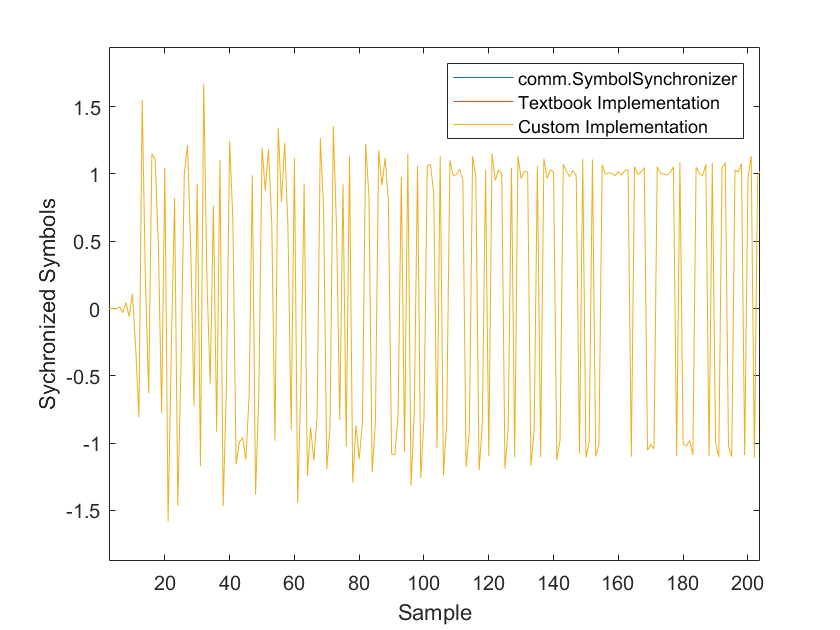
\includegraphics[width=0.5\textwidth]{symbol_sync_no_noise.png}}}
	\caption{Comparison of Synchronized Symbols}
	\label{fig::symbol_sync_no_noise}
\end{figure}

\begin{figure}[H]
	\centerline{\fbox{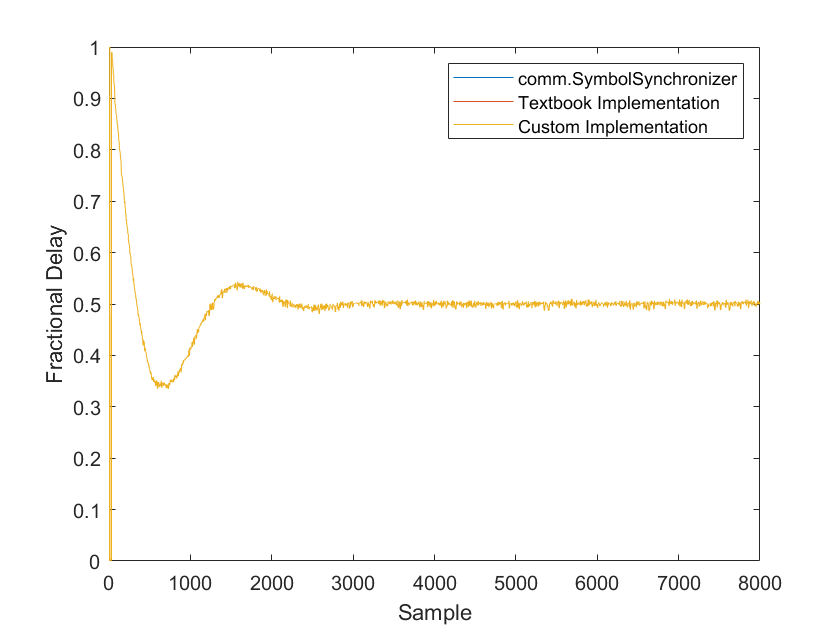
\includegraphics[width=0.5\textwidth]{fractional_delay_no_noise.png}}}
	\caption{Comparison of Fractional Delay}
	\label{fig::fractional_delay_no_noise}
\end{figure}

\noindent Comparing the outputs of each routine, we see that the routine outputs are approximately the same, indicating a correct implementation. We also see that the loop filter parameters cause the fractional delay to converge. For completeness, we also plot the error between the \texttt{comm.SymbolSynchronizer} outputs and the custom routine outputs, which we have included in Figures \ref{fig::symbol_sync_error} and \ref{fig::fractional_delay_error}.

\begin{figure}[H]
	\centerline{\fbox{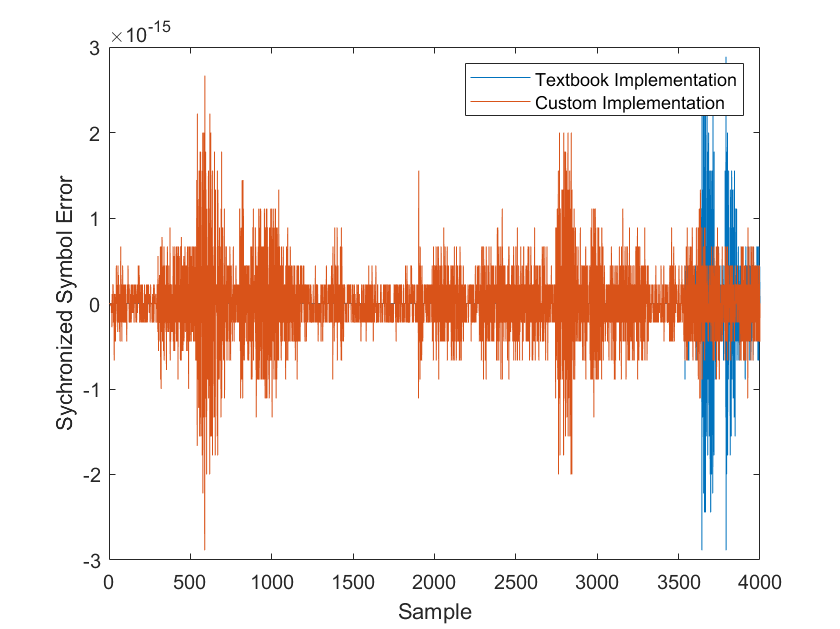
\includegraphics[width=0.5\textwidth]{symbol_sync_error.png}}}
	\caption{Comparison of Synchronized Symbols}
	\label{fig::symbol_sync_error}
\end{figure}

\begin{figure}[H]
	\centerline{\fbox{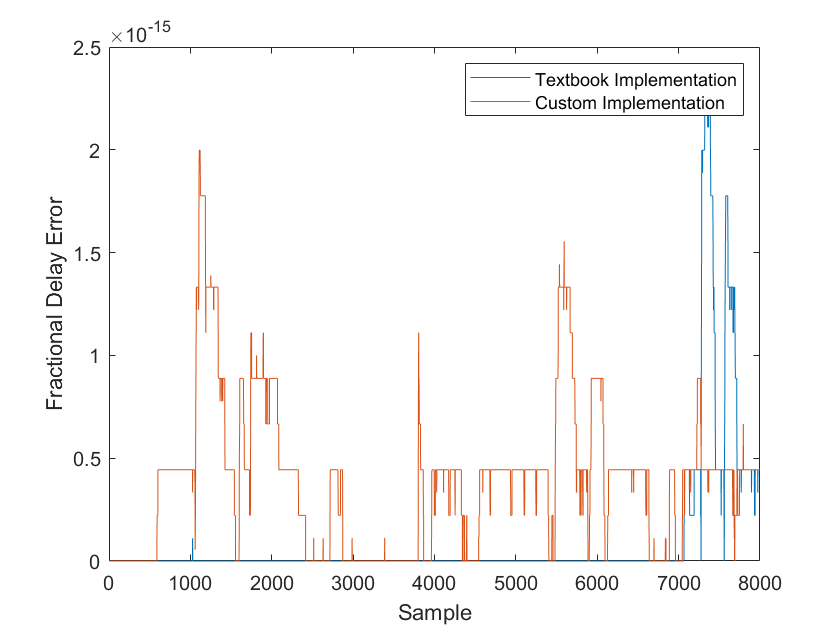
\includegraphics[width=0.5\textwidth]{fractional_delay_error.png}}}
	\caption{Comparison of Fractional Delay}
	\label{fig::fractional_delay_error}
\end{figure}

\noindent With respect to the signal amplitudes, the errors are effectively zero. Therefore, we conclude that our custom implementations are implemented correctly. We also examine the error signal ($e(n)$) output by the zero-crossing timing error detector. This value is not output by the \texttt{comm.SymbolSynchronizer}. However, we can examine it for each of our implementations.  We have plotted this error signal in Figure \ref{fig::timing_offset}. 

\begin{figure}[H]
	\centerline{\fbox{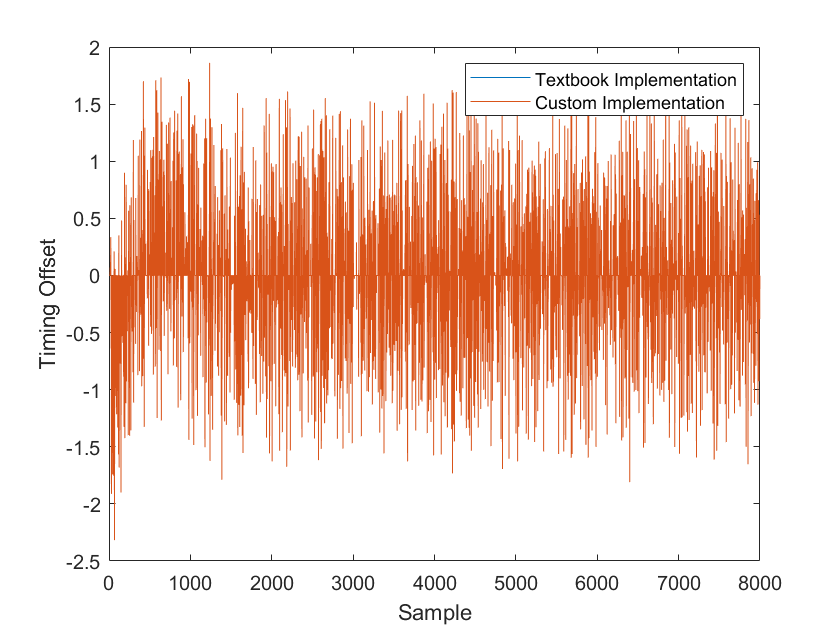
\includegraphics[width=0.5\textwidth]{timing_offset.png}}}
	\caption{Error Signal Output by ZC TED}
	\label{fig::timing_offset}
\end{figure}

\noindent Examining the timing offsets, we see that the both routines output the same values. We can also draw a few other conclusions. First, we see that the error signal alternates between zero and non-zero values. This is expected because the timing error detector only outputs non-zero values when it receives a trigger, which happens roughly every other cycle. Additionally, we see that the timing offset rapidly oscillates even after the fractional delay has converged. However, we have previously shown that this is not an error because the fractional delay converges and because the results are consistent with the \texttt{comm.SymbolSynchronizer}.

A better indication of the PLL performance is the fractional delay error (i.e. the difference between the measured fractional delay and configured fractional delay). Figure \ref{fig::delay_error_no_noise} display this error for a noise-free signal, and Figures \ref{fig::delay_error_20dB_snr} and \ref{fig::delay_error_10dB_snr} display this error for 20dB and 10dB SNR respectively. 

\begin{figure}[H]
	\centerline{\fbox{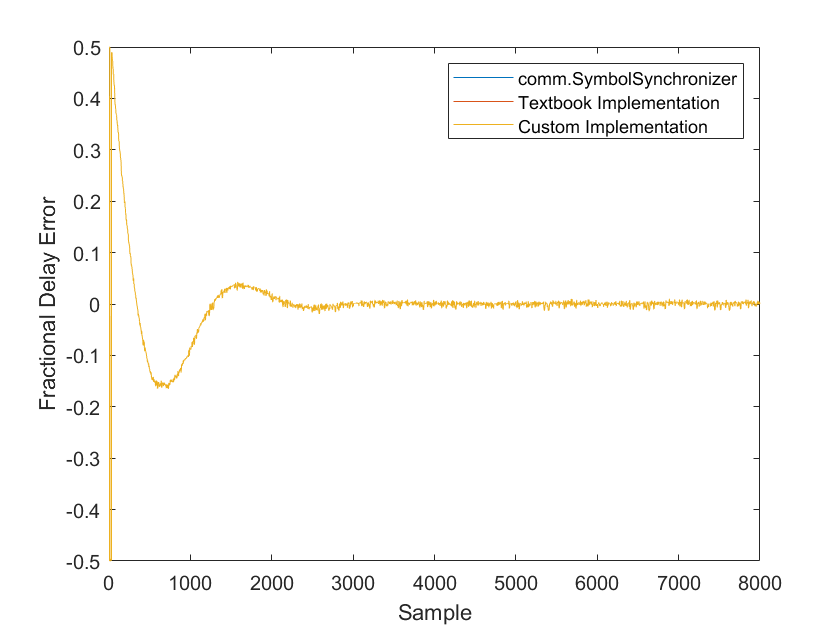
\includegraphics[width=0.5\textwidth]{delay_error_no_noise.png}}}
	\caption{Fractional Delay Error for Noise Free Signal}
	\label{fig::delay_error_no_noise}
\end{figure}

\begin{figure}[H]
	\centerline{\fbox{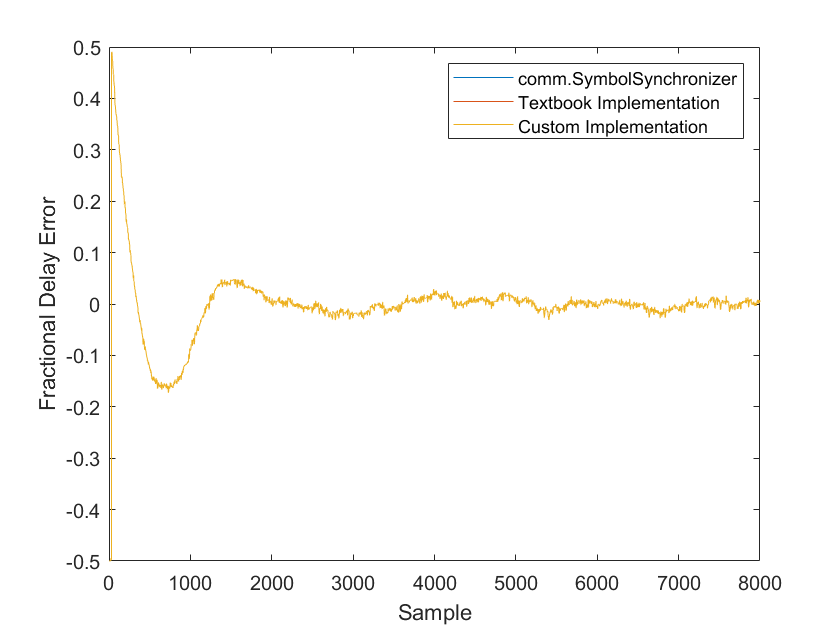
\includegraphics[width=0.5\textwidth]{delay_error_20dB_snr.png}}}
	\caption{Fractional Delay Error for Signal with 20dB SNR}
	\label{fig::delay_error_20dB_snr}
\end{figure}

\begin{figure}[H]
	\centerline{\fbox{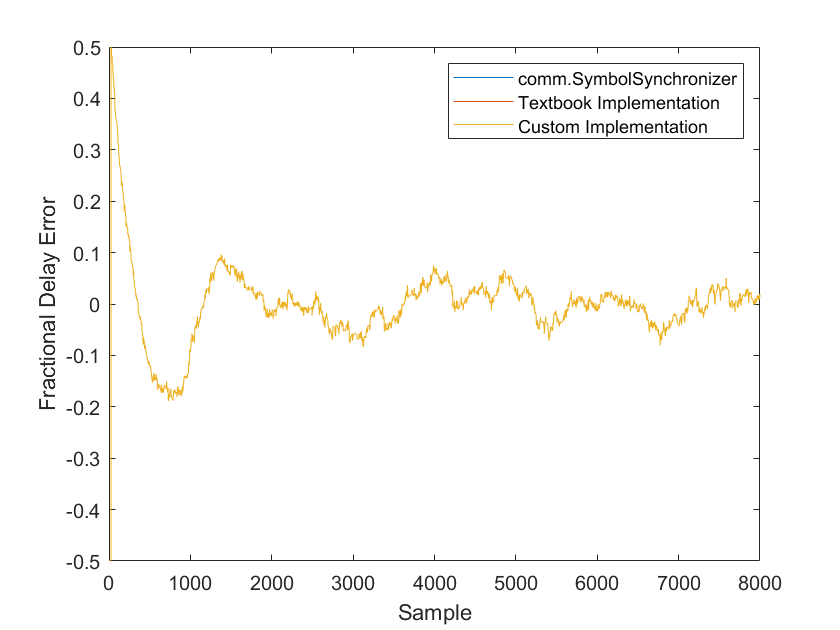
\includegraphics[width=0.5\textwidth]{delay_error_10dB_snr.png}}}
	\caption{Fractional Delay Error for Signal with 10dB SNR}
	\label{fig::delay_error_10dB_snr}
\end{figure}

\noindent Comparing each of the figures, we see that the timing compensation is dependent on the SNR of the received signal (better SNR leads to better timing compensation). Additionally, across a range of SNRs, the custom routines produce results that are consistent with MATLAB's \texttt{comm.SymbolSynchronizer}.

\subsubsection{Performance}

Next, we analyze the performance of the timing compensation logic when we apply a slowly-changing timing offset. For this experiment, we specifically allow the timing offset to drift by a hundredth of symbol every 1024 symbols. In Figure \ref{fig::fractional_delay_timing_offset}, we show the measured fractional delay with a 20 dB SNR, and in Figure \ref{fig::fractional_delay_error_timing_offset}, we show the fractional delay error.

\begin{figure}[H]
	\centerline{\fbox{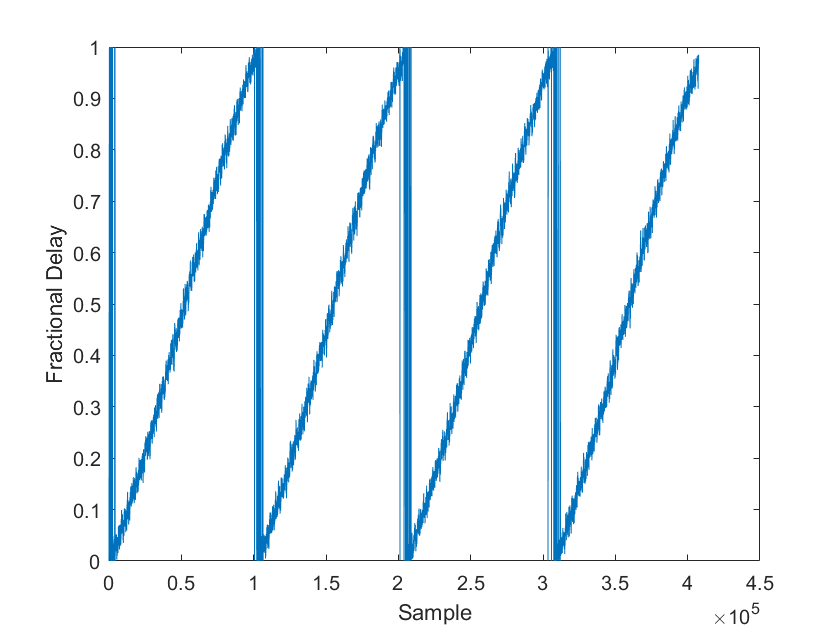
\includegraphics[width=0.5\textwidth]{fractional_delay_timing_offset.png}}}
	\caption{Fractional Delay Measured for Data with Slowly Varying Timing Delay}
	\label{fig::fractional_delay_timing_offset}
\end{figure}

\begin{figure}[H]
	\centerline{\fbox{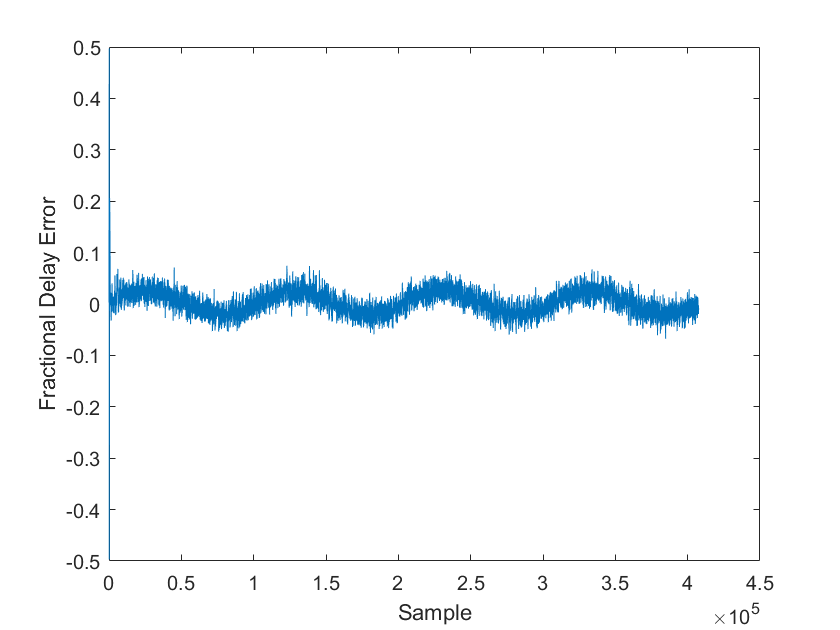
\includegraphics[width=0.5\textwidth]{fractional_delay_error_timing_offset.png}}}
	\caption{Fractional Delay Error Measured for Data with Slowly Varying Timing Delay}
	\label{fig::fractional_delay_error_timing_offset}
\end{figure}

\noindent Examining the figure outputs, we see that the fractional delay increases linearly with time as expected. Additionally, we see that the timing error converges to zero. However, compared to the outputs shown in Figures \ref{fig::delay_error_no_noise}, the fractional delay error oscillates at steady state. In Figure \ref{fig::constellations_with_timing_correction}, we show the constellations before and after timing compensation. For this analysis, we use BPSK modulation.
 
\begin{figure}[H]
	\centerline{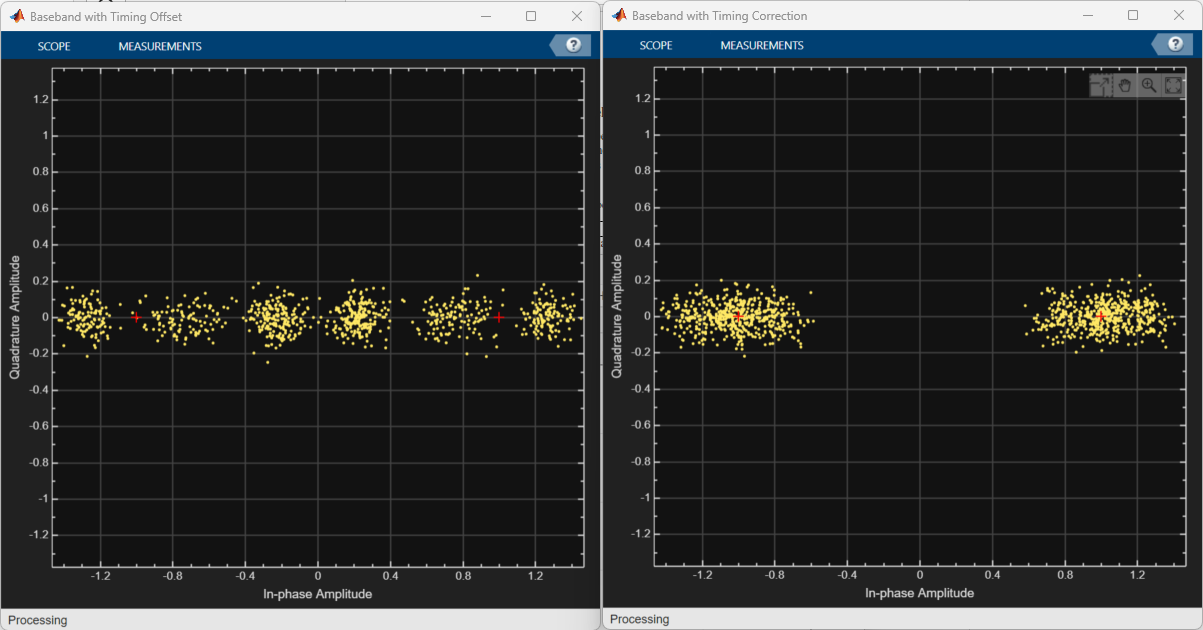
\includegraphics[width=0.8\textwidth]{constellations_with_timing_correction.png}}
	\caption{Constellations Before Timing Compensation (Left) and After Timing Compensation (Right)}
	\label{fig::constellations_with_timing_correction}
\end{figure}

\noindent Before timing compensation, the constellation does not match closely with our expectations for BPSK modulation. However, after timing compensation, all the received data is clustered around $\pm 1$ as expected.

We can quantify how closely our constellation matches the desired constellation by examining the error vector magnitude (EVM). In Figures \ref{fig::evm_vs_snr_no_correction} and \ref{fig::evm_vs_snr}, we plot the EVM of the data against SNR. Figure \ref{fig::evm_vs_snr_no_correction} shows the EVM prior to timing correction, Figure \ref{fig::evm_vs_snr}, shows the EVM after timing correction. 

\begin{figure}[H]
	\centerline{\fbox{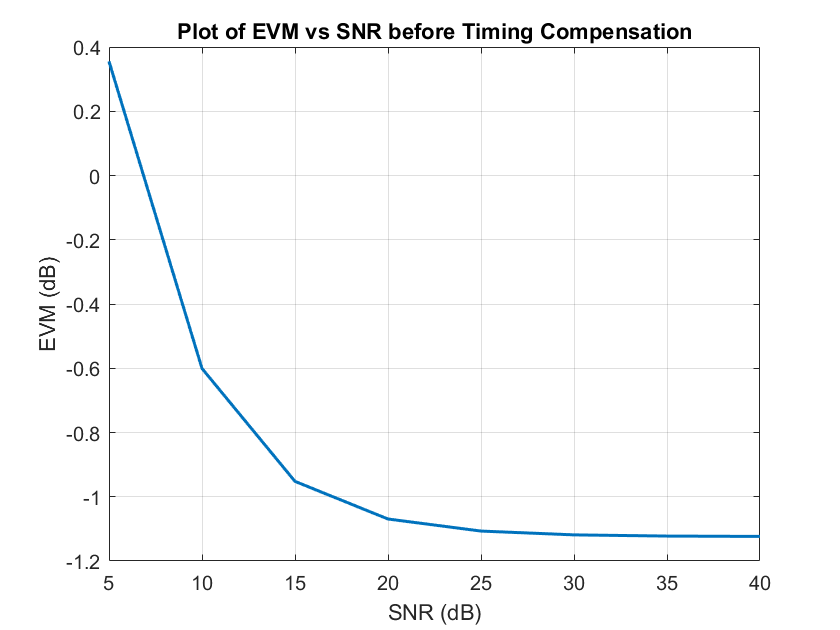
\includegraphics[width=0.5\textwidth]{evm_vs_snr_no_correction.png}}}
	\caption{Plot of EVM vs SNR before Timing Compensation}
	\label{fig::evm_vs_snr_no_correction}
\end{figure}

\begin{figure}[H]
	\centerline{\fbox{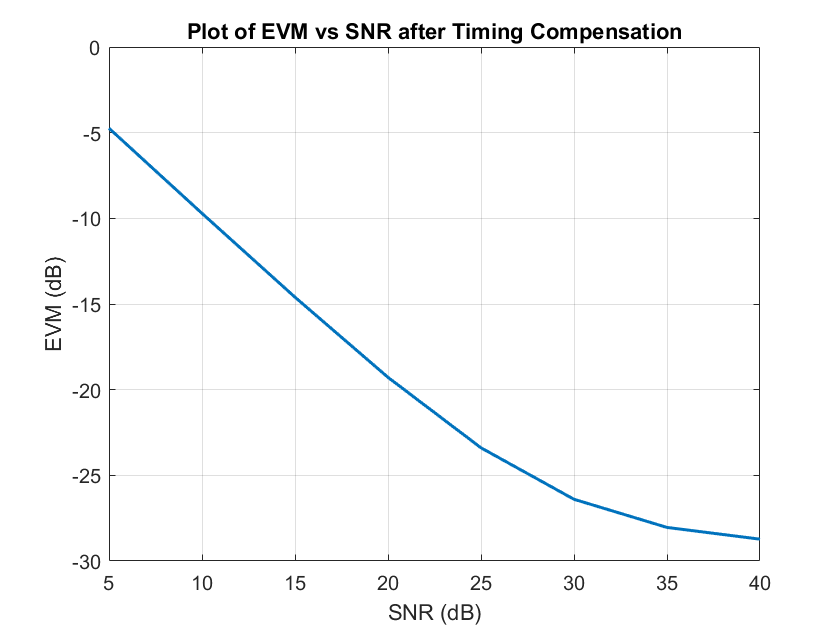
\includegraphics[width=0.5\textwidth]{evm_vs_snr.png}}}
	\caption{Plot of EVM vs SNR after Timing Compensation}
	\label{fig::evm_vs_snr}
\end{figure}

Comparing the plots, we see that the EVM is substantially lower after timing compensation. This is consistent with out qualitative analysis of the constellation. Additionally, we find that the EVM falls with SNR. This is also an expected result because the spread of the constellation points reduces as the SNR increases. Additionally, for low SNRs, we see that the EVM after timing compensation is approximately the -SNR. This phenomenon occurs because the constellation error at low SNRs is dominated by the noise. As the SNR increases, our EVM with timing compensation converges to about -16 dB. In this simulation, the minimum EVM is primarily limited by the drift of our timing offset.

	We can perform similar analysis after adding a phase offset of $\pi/8$ radians. The EVMs before and after timing compensation are included in Figures \ref{fig::evm_vs_snr_with_phase_offset} and \ref{fig::evm_vs_snr_with_phase_offset} respectively.

\begin{figure}[H]
	\centerline{\fbox{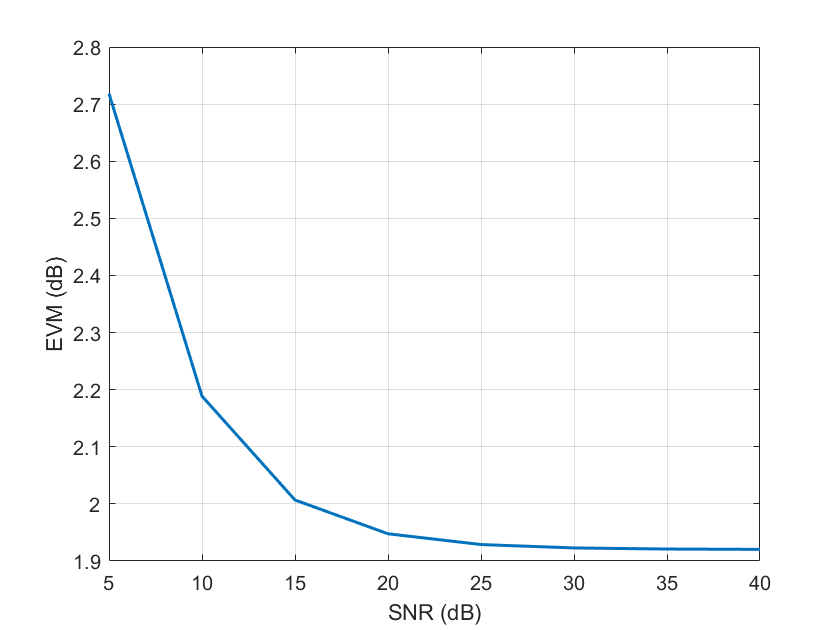
\includegraphics[width=0.5\textwidth]{evm_vs_snr_with_phase_offset_no_comp.png}}}
	\caption{Plot of EVM vs SNR with $\protect\pi/8$ Phase Offset and no Timing Compensation}
	\label{fig::evm_vs_snr_with_phase_offset_no_comp}
\end{figure}

\begin{figure}[H]
	\centerline{\fbox{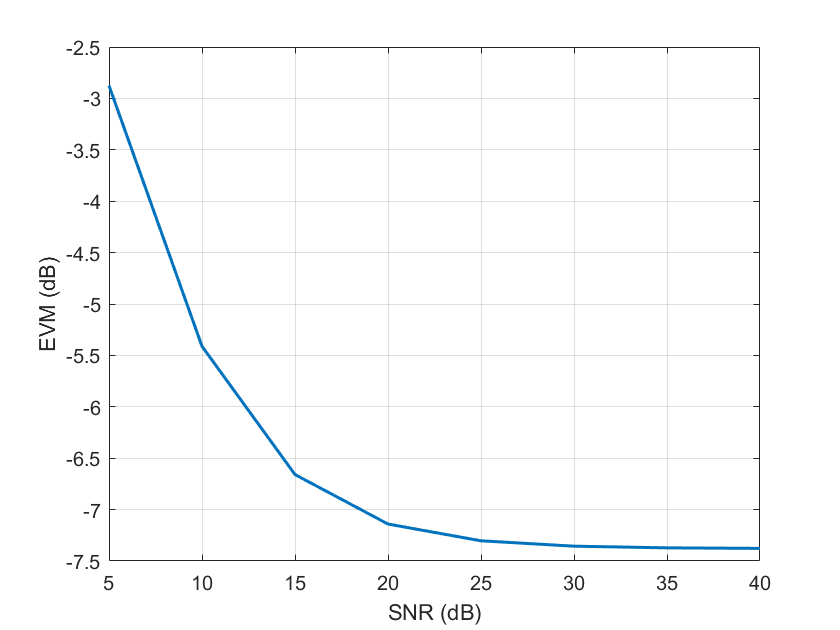
\includegraphics[width=0.5\textwidth]{evm_vs_snr_with_phase_offset.png}}}
	\caption{Plot of EVM vs SNR with $\protect\pi/8$ Phase Offset and Timing Compensation}
	\label{fig::evm_vs_snr_with_phase_offset}
\end{figure}

\noindent Comparing both of our Figures, we see that the EVM of the constellation prior to timing compensation is worse than the EVM after timing compensation. Additionally, compared to our results without a phase offset, we see that our EVM has increased. For the constellation with timing correction, our EVM is almost 10 dB worse in steady state. Our minimum EVM is now limited by the phase offset. With perfect timing compensation and no noise our minimum error with a $\pi/8$ phase offset is limited to

\begin{equation}
	\text{error} = (1 - \cos\pi/8)^2 + \sin^2\pi/8 = 1 - 2\cos\pi/8 + \cos^2\pi/8 + \sin^2\pi/8 = 2 - 2\cos\pi/8 \approx 0.15224 
\end{equation}

\noindent which corresponds to an EVM of 

\begin{equation}
	\text{EVM}_{\text{dB}} = 10\log_{10}\left(\text{error}\right) \approx 10\log_{10}(0.15224) \approx -8.17\ \text{dB}
\end{equation}

\noindent Note that our EVM curve does not hit this minimum value because of timing drift, which leads to timing errors (even after compensation). We can look at the constellations shown in Figure \ref{fig::constellations_with_timing_correction_phase_offset}, to visualize the effects of the phase offset.

\begin{figure}[H]
	\centerline{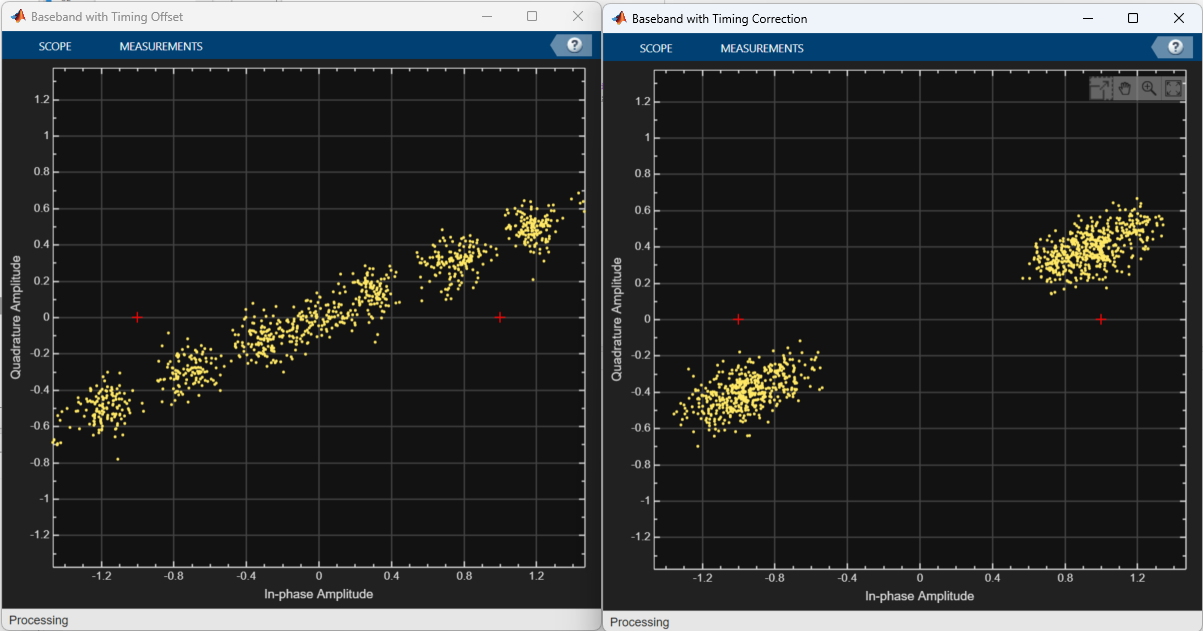
\includegraphics[width=0.8\textwidth]{constellations_with_timing_correction_phase_offset.png}}
	\caption{Constellations with Phase Offset Before and After Timing Compensation}
	\label{fig::constellations_with_timing_correction_phase_offset}
\end{figure}

\noindent Examining the figure, we see that the timing compensation correctly clusters each of the received symbols. However, the symbols have been rotated due to phase error. To account for the phase error, we can use differential modulation (DBPSK vs BPSK). For our DBPSK demodulation, we use the phase difference between adjacent samples to determine the transmitted symbols. We can use the following equation to examine the constellation points after differential demodulation:

\begin{equation}
	y[n] = A[n]e^{j\phi[n]}*e^{-j\phi[n-1]}
	\label{eq::dbpsk}
\end{equation}

\noindent Using the updated constellation points, we compute the EVM before and after timing compensation. We plot these results in Figures \ref{fig::evm_vs_snr_dbpsk_no_comp} and \ref{fig::evm_vs_snr_dbpsk}.

\begin{figure}[H]
	\centerline{\fbox{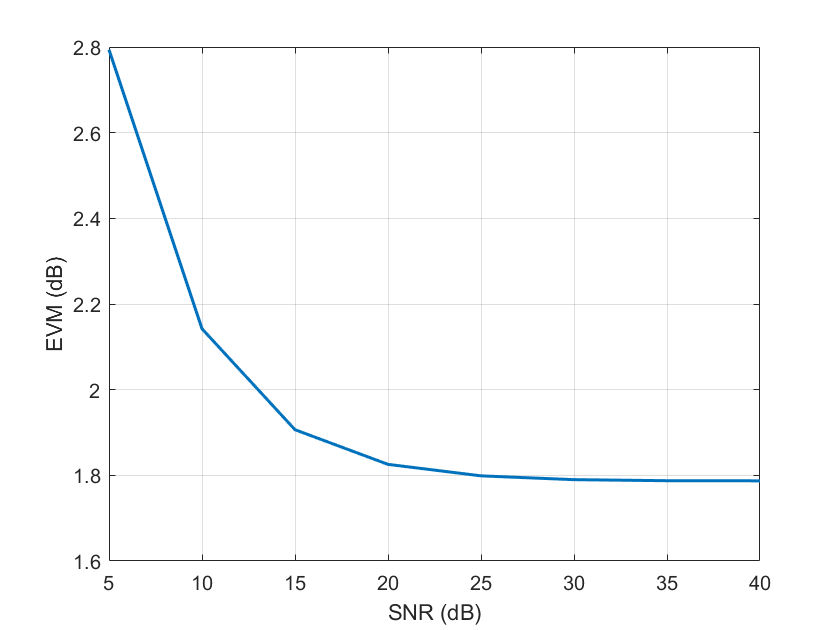
\includegraphics[width=0.5\textwidth]{evm_vs_snr_dbpsk_no_comp.png}}}
	\caption{Plot of EVM vs SNR with DBPSK Modulation and no Timing Compensation}
	\label{fig::evm_vs_snr_dbpsk_no_comp}
\end{figure}

\begin{figure}[H]
	\centerline{\fbox{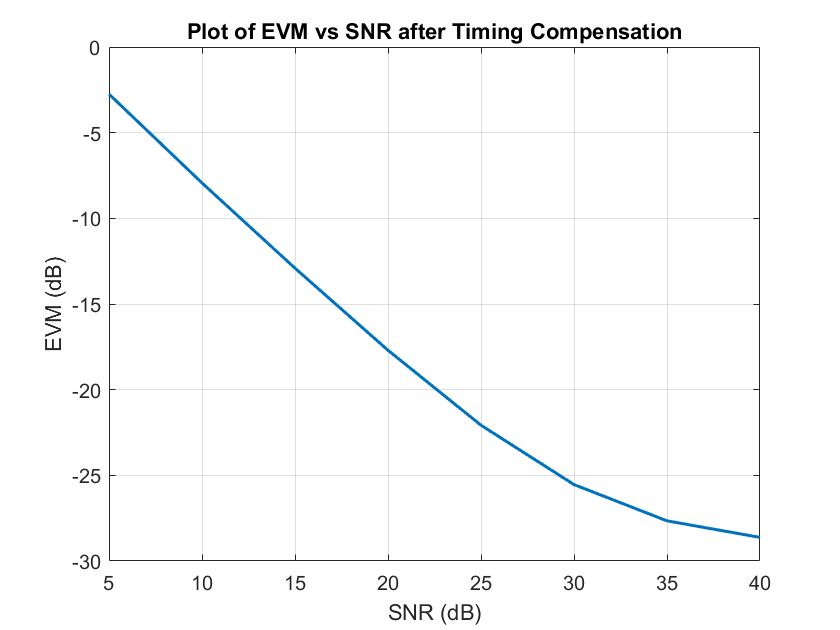
\includegraphics[width=0.5\textwidth]{evm_vs_snr_dbpsk.png}}}
	\caption{Plot of EVM vs SNR with DPSK Modulation and Timing Compensation}
	\label{fig::evm_vs_snr_dbpsk}
\end{figure}

Compared to our results with BPSK modulation, we see that the EVM with timing compensation has substantially improved, getting close to the no phase offset case. At low SNRs, the EVM is slightly worse because we use noisy samples in our differential demodulation.

\subsection{Adding Pieces Together}
\label{section::adding_pieces_together}

In this section, we review the timing recovery circuit and the sample rates of each of its blocks. A block diagram of the timing recovery circuit is included in Figure \ref{fig::timing_recovery_block_diagram_2}. Our timing recovery circuit (with the exception of the "asynchronous FIFO" interface) runs at a sample rate of $2/T_s$, where $T_s$ is the symbol duration. As a result, our receive filter must output samples at twice the symbol rate.

	The interpolator receives a fractional delay, which is updated each trigger. It outputs the signal with fractional delay and delayed-version of the trigger to an "asynchronous FIFO" interface. This FIFO stores the filter output every time it receives a trigger and outputs 1 sample per symbol. Triggers occur on average once per cycle as well, so there is little risk of overflow. To the ensure the design is resilient, we may clear the FIFO if it starts to overflow. However, this feature is not included in our implementation.
	
	The timing error detector implements the zero-crossing algorithm. As such, it requires an additional interpolator, which is not shown. The timing error detector outputs an error every time it receives a trigger. When it does not receive a trigger, the timing error detector outputs a zero. The loop filter uses a PI filter and provides stimulus to the interpolation controller, which, in turn, creates triggers and updates the fractional delay parameter.
	
\begin{figure}[H]
	\centerline{\fbox{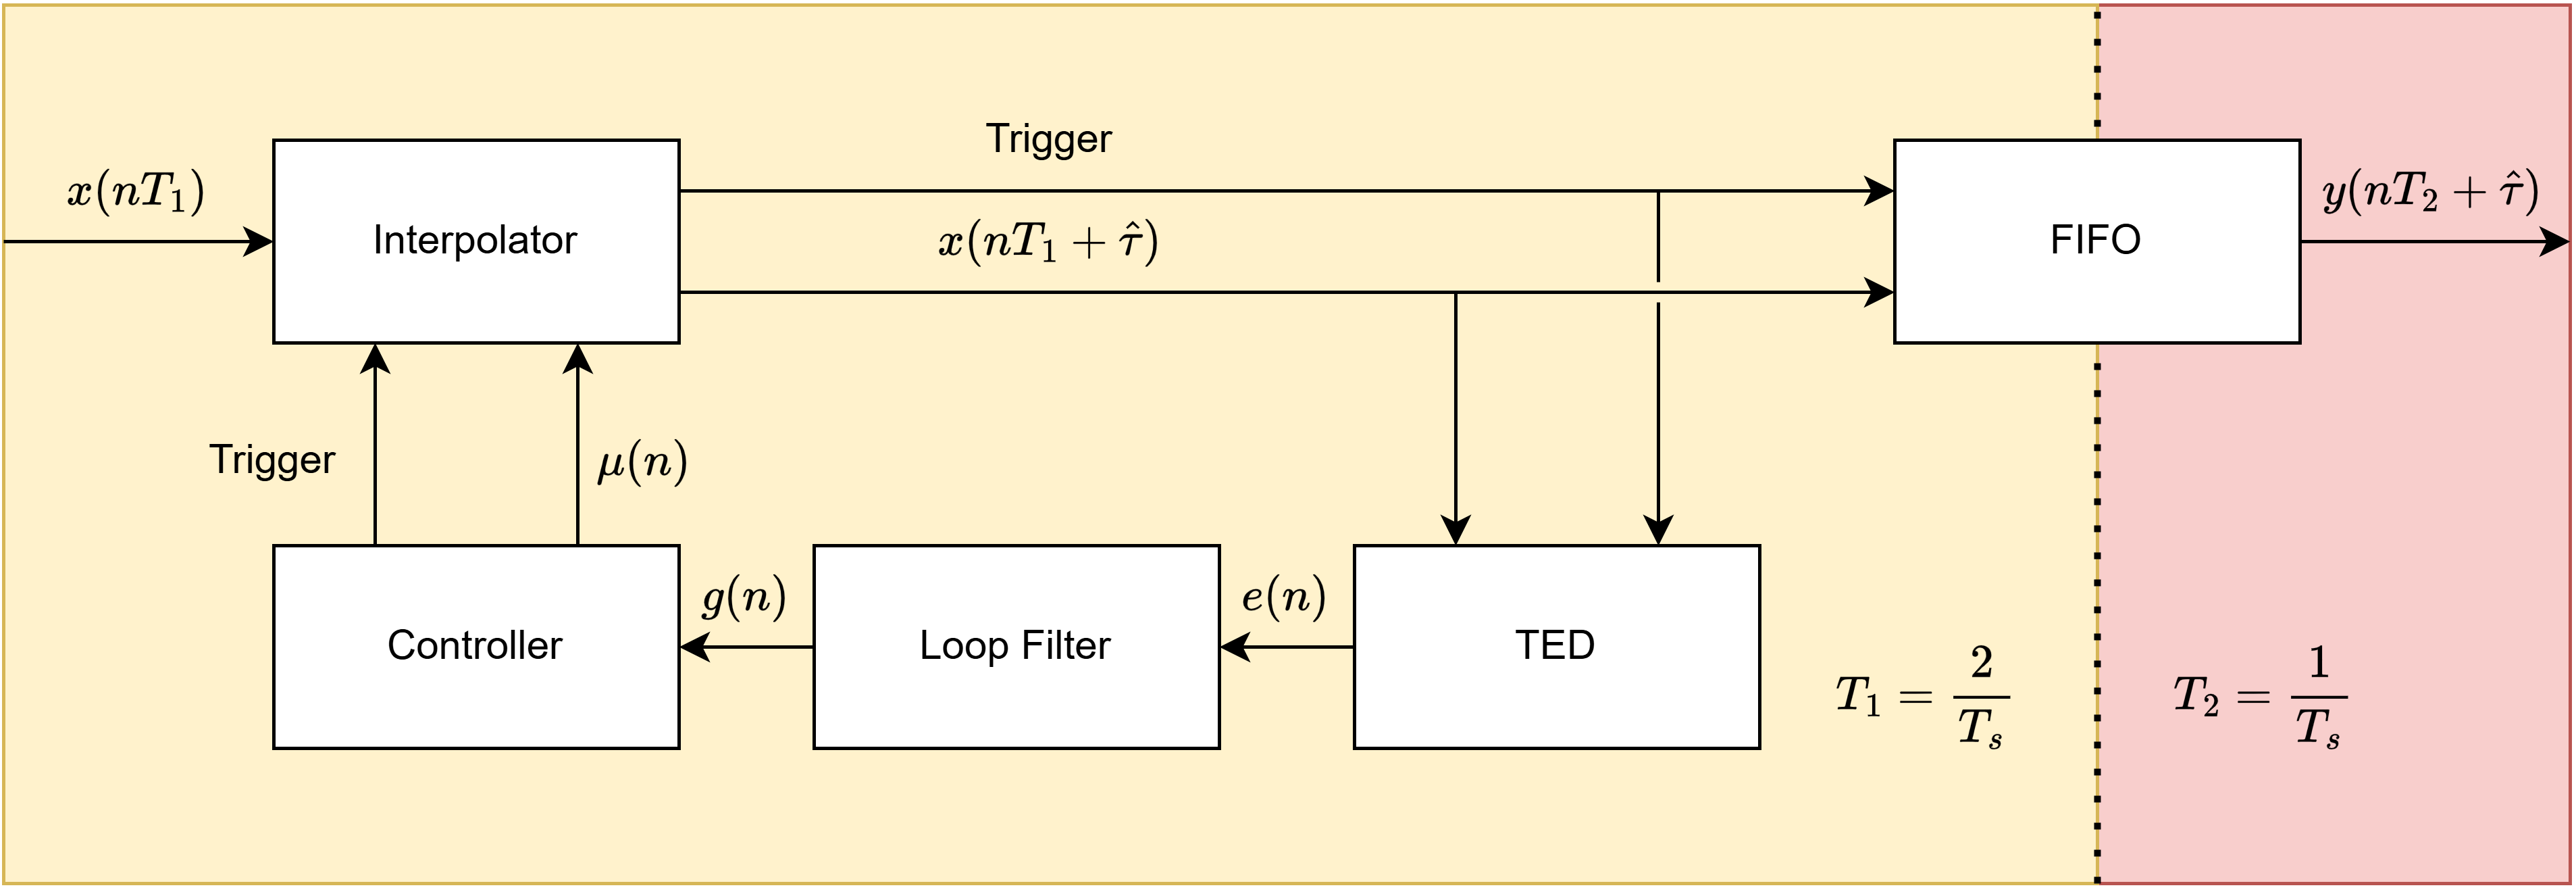
\includegraphics[width=0.7\textwidth]{timing_recovery_block_diagram_2.png}}}
	\caption{Block Diagram of Timing Recovery Circuit}
	\label{fig::timing_recovery_block_diagram_2}
\end{figure}

We evaluate the performance of the timing recovery block by measuring the EVM under a couple different conditions. First we measure the EVM with no timing offsets (i.e. the ideal base case). These results are included in Figures \ref{fig::evm_no_timing_offset} and \ref{fig::evm_no_timing_offset}.

\begin{figure}[H]
	\centerline{\fbox{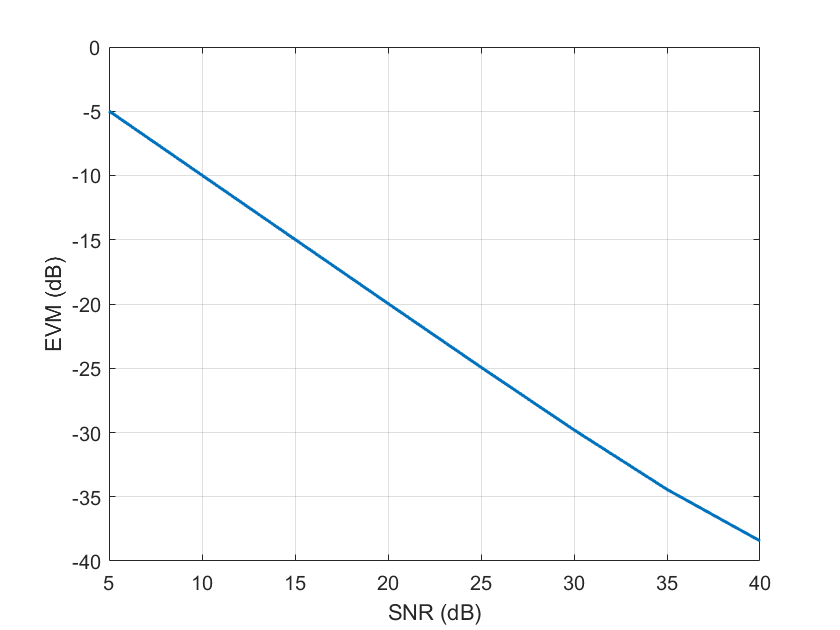
\includegraphics[width=0.5\textwidth]{evm_no_timing_offset_no_comp.png}}}
	\caption{Plot of EVM vs SNR with No Timing Offsets or Timing Compensation}
	\label{fig::evm_no_timing_offset_no_comp}
\end{figure}

\begin{figure}[H]
	\centerline{\fbox{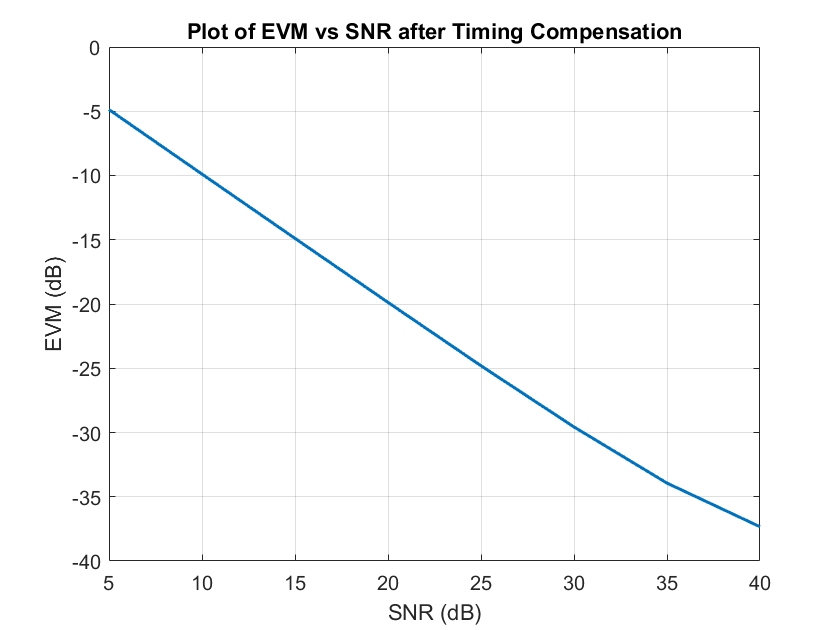
\includegraphics[width=0.5\textwidth]{evm_no_timing_offset.png}}}
	\caption{Plot of EVM vs SNR with No Timing Offsets and Timing Compensation}
	\label{fig::evm_no_timing_offset}
\end{figure}

Comparing both figures, we see that the EVM is roughly the same with and without timing compensation. This is the expected result because there is no timing offset. Additionally, we see that EVM is approximately the same as -SNR in both cases. This is also an expected result because the EVM is measuring the error power (noise power) over the constellation power (signal power). Next, we consider the EVM when we apply a fixed timing offset of $0.25T_s$. These results are included in Figures \ref{fig::evm_0p25_symbol_offset_no_comp} and \ref{fig::evm_0p25_symbol_offset}.

\begin{figure}[H]
	\centerline{\fbox{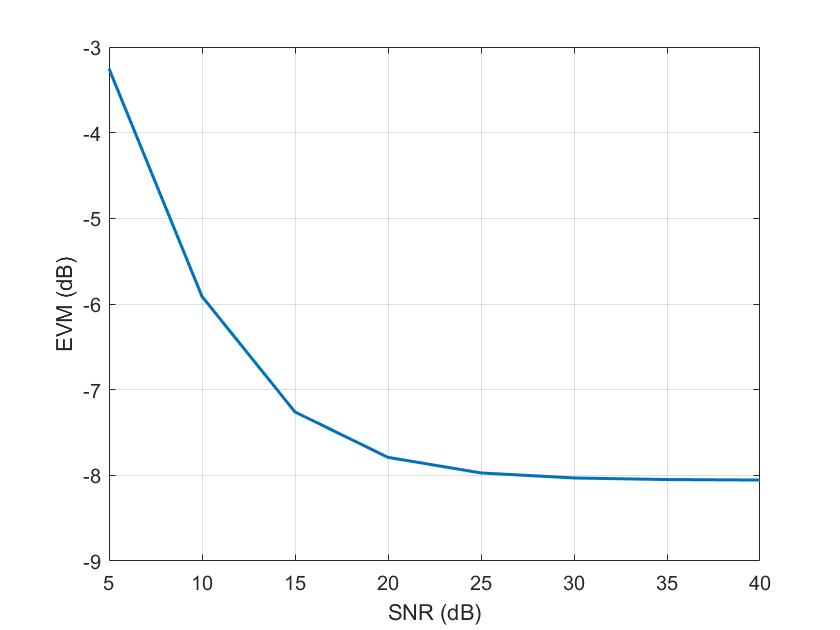
\includegraphics[width=0.5\textwidth]{evm_0p25_symbol_offset_no_comp.png}}}
	\caption{Plot of EVM vs SNR with $\protect{0.25T_s}$ Symbol Offset and No Timing Compensation}
	\label{fig::evm_0p25_symbol_offset_no_comp}
\end{figure}

\begin{figure}[H]
	\centerline{\fbox{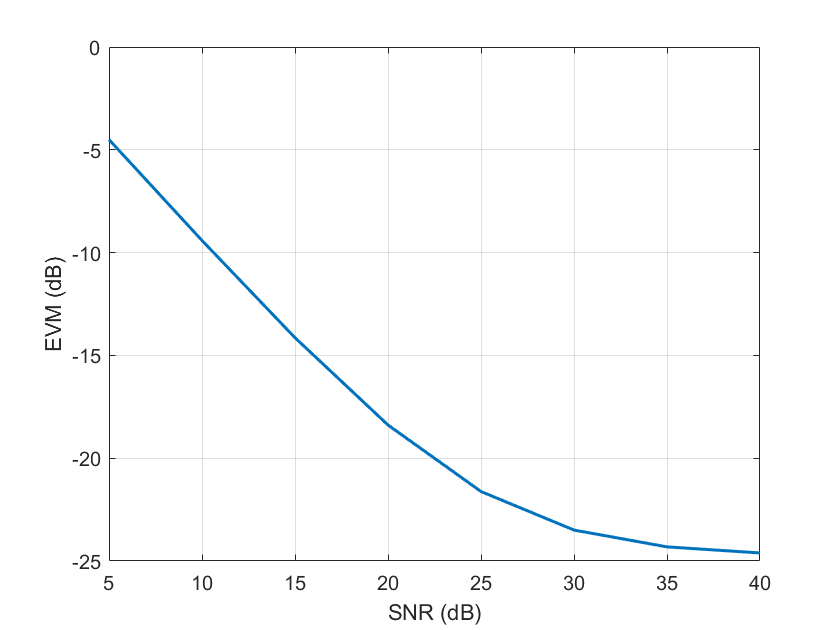
\includegraphics[width=0.5\textwidth]{evm_0p25_symbol_offset.png}}}
	\caption{Plot of EVM vs SNR with $\protect{0.25T_s}$ Symbol Offset and Timing Compensation}
	\label{fig::evm_0p25_symbol_offset}
\end{figure}

Examining the figures, we see that the EVM without timing compensation is substantially degraded. However, after timing compensation, the EVM improves significantly. At low SNR's it is approximately, the no timing error case. However, as the SNR increases, the timing recovery circuit limits the minimum EVM to about -25 dB. This is slightly better than the results shown in Figure \ref{fig::evm_vs_snr} because the timing offset does not drift with time. Next, we examine the performance when we apply a phase offset of $\pi/4$ radians instead of a timing error. These results are included in Figures \ref{fig::evm_pi_4_phase_offset_no_comp} and \ref{fig::evm_pi_4_phase_offset}.

\begin{figure}[H]
	\centerline{\fbox{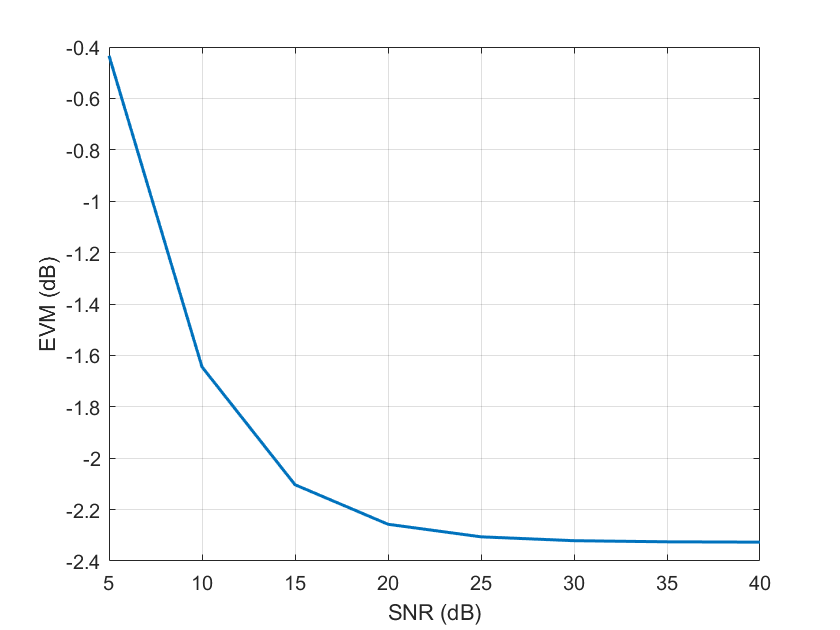
\includegraphics[width=0.5\textwidth]{evm_pi_4_phase_offset.png}}}
	\caption{Plot of EVM vs SNR with $\protect\pi/4$ Phase Offset and No Timing Compensation}
	\label{fig::evm_pi_4_phase_offset_no_comp}
\end{figure}

\begin{figure}[H]
	\centerline{\fbox{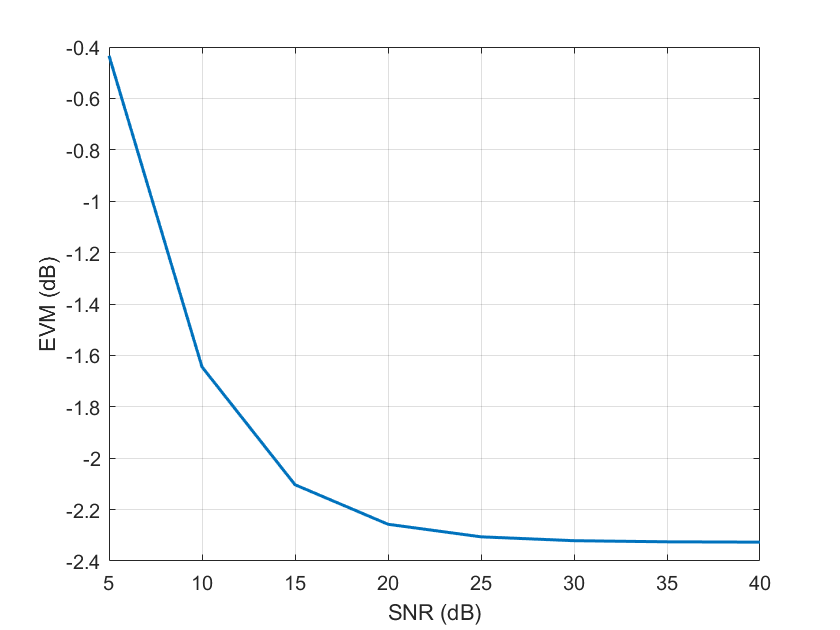
\includegraphics[width=0.5\textwidth]{evm_pi_4_phase_offset.png}}}
	\caption{Plot of EVM vs SNR with $\protect\pi/4$ Phase Offset and Timing Compensation}
	\label{fig::evm_pi_4_phase_offset}
\end{figure}

Comparing the results of both Figures, we see that the timing compensation logic does not improve the EVM when we have a phase offset. At high SNR, the minimum error converges to

\begin{equation}
	\text{error} = (1 - \cos\pi/4)^2 + \sin^2\pi/4 = 1 - 2\cos\pi/4 + \cos^2\pi/4 + \sin^2\pi/4 = 2 - 2\cos\pi/4 \approx 0.58578 
\end{equation}

\noindent which corresponds to an EVM of 

\begin{equation}
	\text{EVM}_{\text{dB}} = 10\log_{10}\left(\text{error}\right) \approx 10\log_{10}(0.58578) \approx -2.32\ \text{dB}
\end{equation}

\noindent Note that this value is consistent with our high-SNR EVM measurement. We can visualize the timing error detector performance in the presence of phase error by examining the constellation, which is shown in Figure \ref{fig::constellation_phase_error}.

\begin{figure}[H]
	\centerline{\fbox{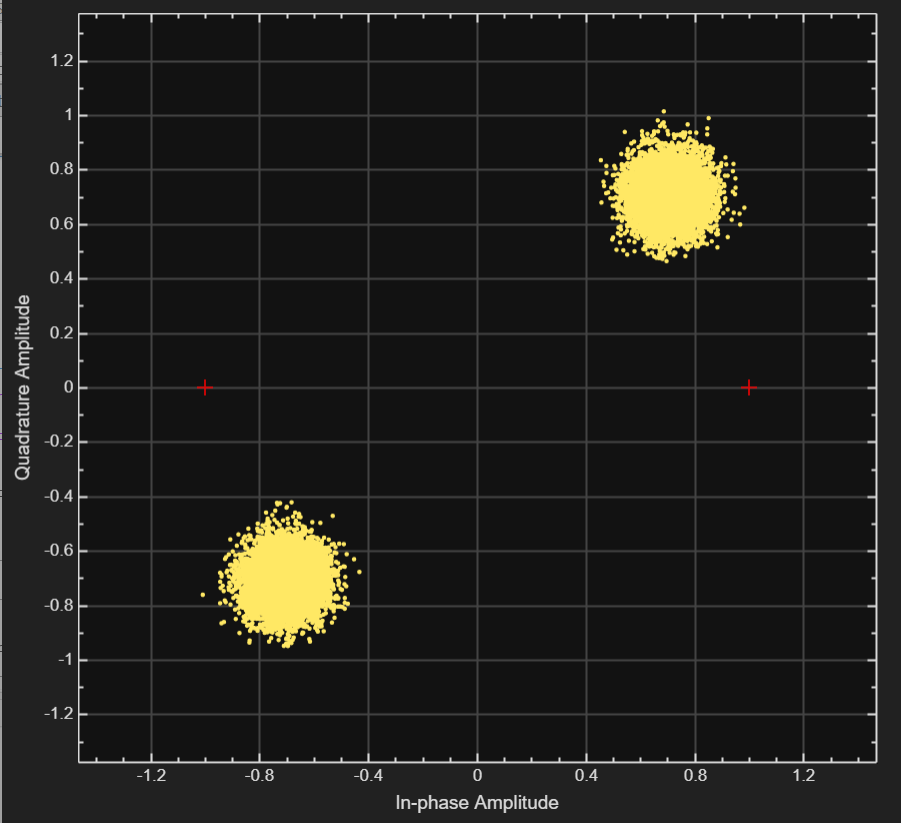
\includegraphics[width=0.5\textwidth]{constellation_phase_error.png}}}
	\caption{Constellation after Timing Compensation with 20 dB SNR and a $\protect\pi/4$ Phase Offset}
	\label{fig::constellation_phase_error}
\end{figure}

\noindent Examining the Figure we see that the phase error creates a rotation in the complex plane, which artificially distorts our EVM metric. One way to handle this phase error is to use differential modulation. We specifically can use DBPSK modulation instead of BPSK modulation. We can specifically use Equation \ref{eq::dbpsk} to access the EVM after DBPSK modulation. The results of this experiment are included in Figures \ref{fig::evm_dpsk_modulation_no_comp} and \ref{fig::evm_dpsk_modulation}.

\begin{figure}[H]
	\centerline{\fbox{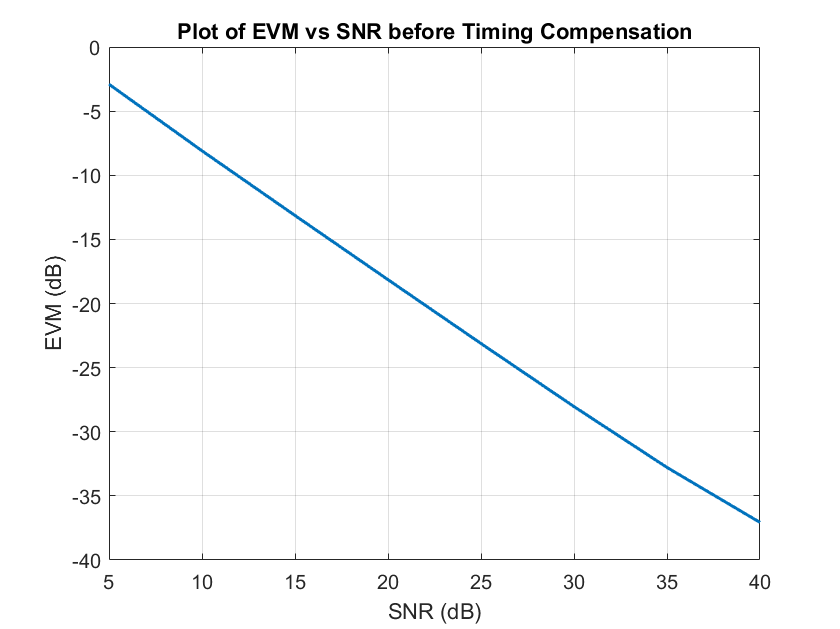
\includegraphics[width=0.5\textwidth]{evm_dpsk_modulation_no_comp.png}}}
	\caption{EVM with $\protect\pi/4$ Phase Offset After Differential Demodulation}
	\label{fig::evm_dpsk_modulation_no_comp}
\end{figure}

\begin{figure}[H]
	\centerline{\fbox{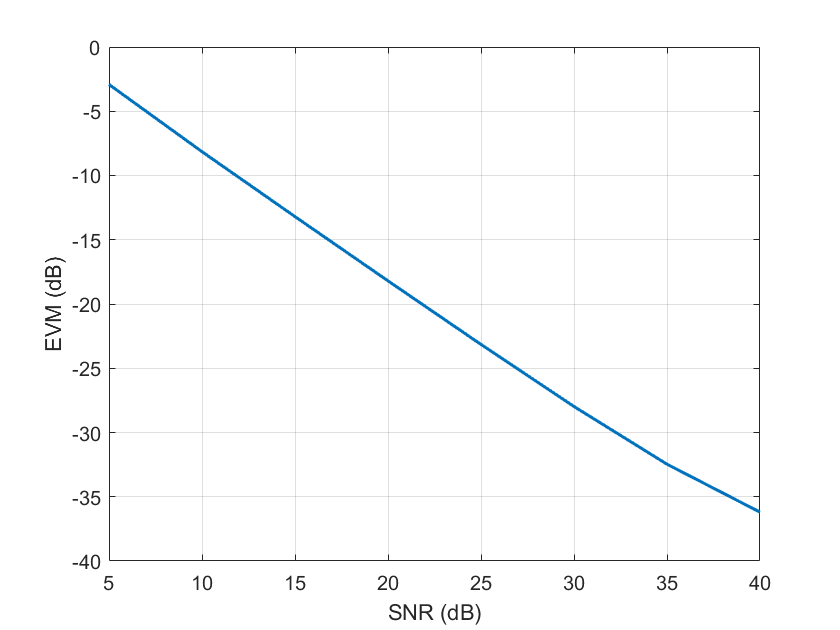
\includegraphics[width=0.5\textwidth]{evm_dpsk_modulation.png}}}
	\caption{EVM with $\protect\pi/4$ Phase Offset After Differential Demodulation}
	\label{fig::evm_dpsk_modulation}
\end{figure}

\noindent Examining the figures, we note that both get close in performance to the baseline case shown in Figures \ref{fig::evm_no_timing_offset_no_comp} and \ref{fig::evm_no_timing_offset}. However, there is some slight degradation in performance because we use noisy samples in our differential demodulation. 

\subsection{Testing on Hardware}

In this section, we perform timing compensation with the PlutoSDR. We start by transmitting BPSK symbols. The resulting constellations before and after timing compensation are included in Figure \ref{fig::pluto_constellations_no_comp}.

\begin{figure}[H]
	\centerline{\fbox{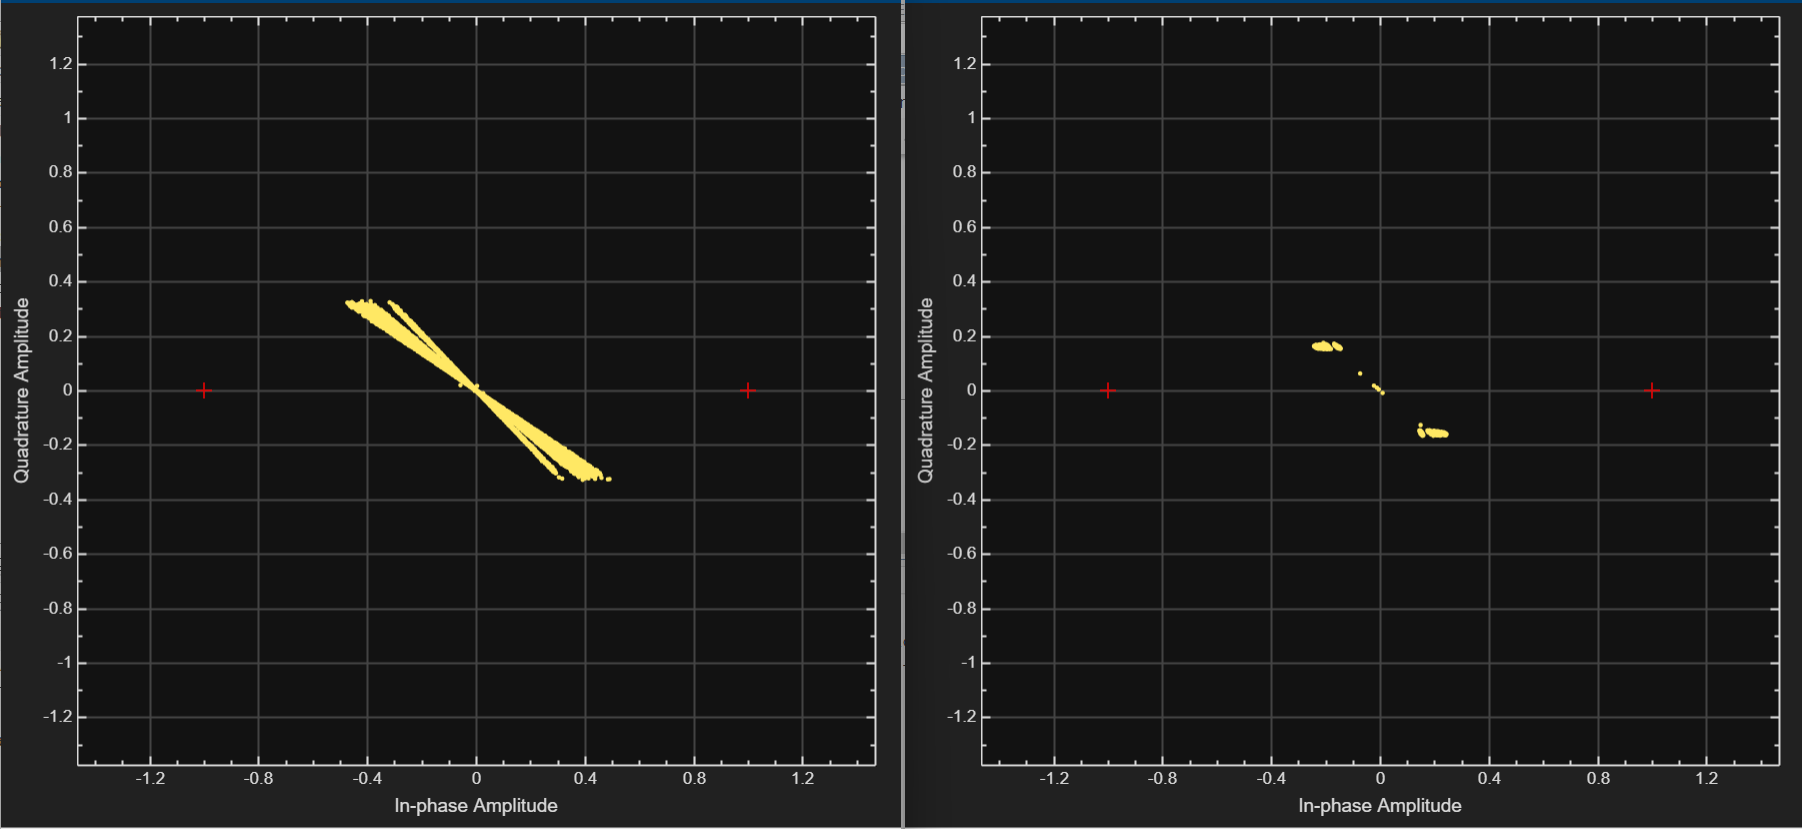
\includegraphics[width=0.7\textwidth]{pluto_constellations_no_comp.png}}}
	\caption{Constellations Collected with PlutoSDR before and after Timing Compensation}
	\label{fig::pluto_constellations_no_comp}
\end{figure}

\noindent Examining the constellations, we observe time, phase, and frequency offsets. The timing compensation only corrects for the timing offsets. However, the phase and frequency offsets still persist. We can use DBPSK modulation to get rid of the phase offsets. The constellations after differential demodulation are shown in Figure \ref{fig::pluto_constellations_dbpsk}.

\begin{figure}[H]
	\centerline{\fbox{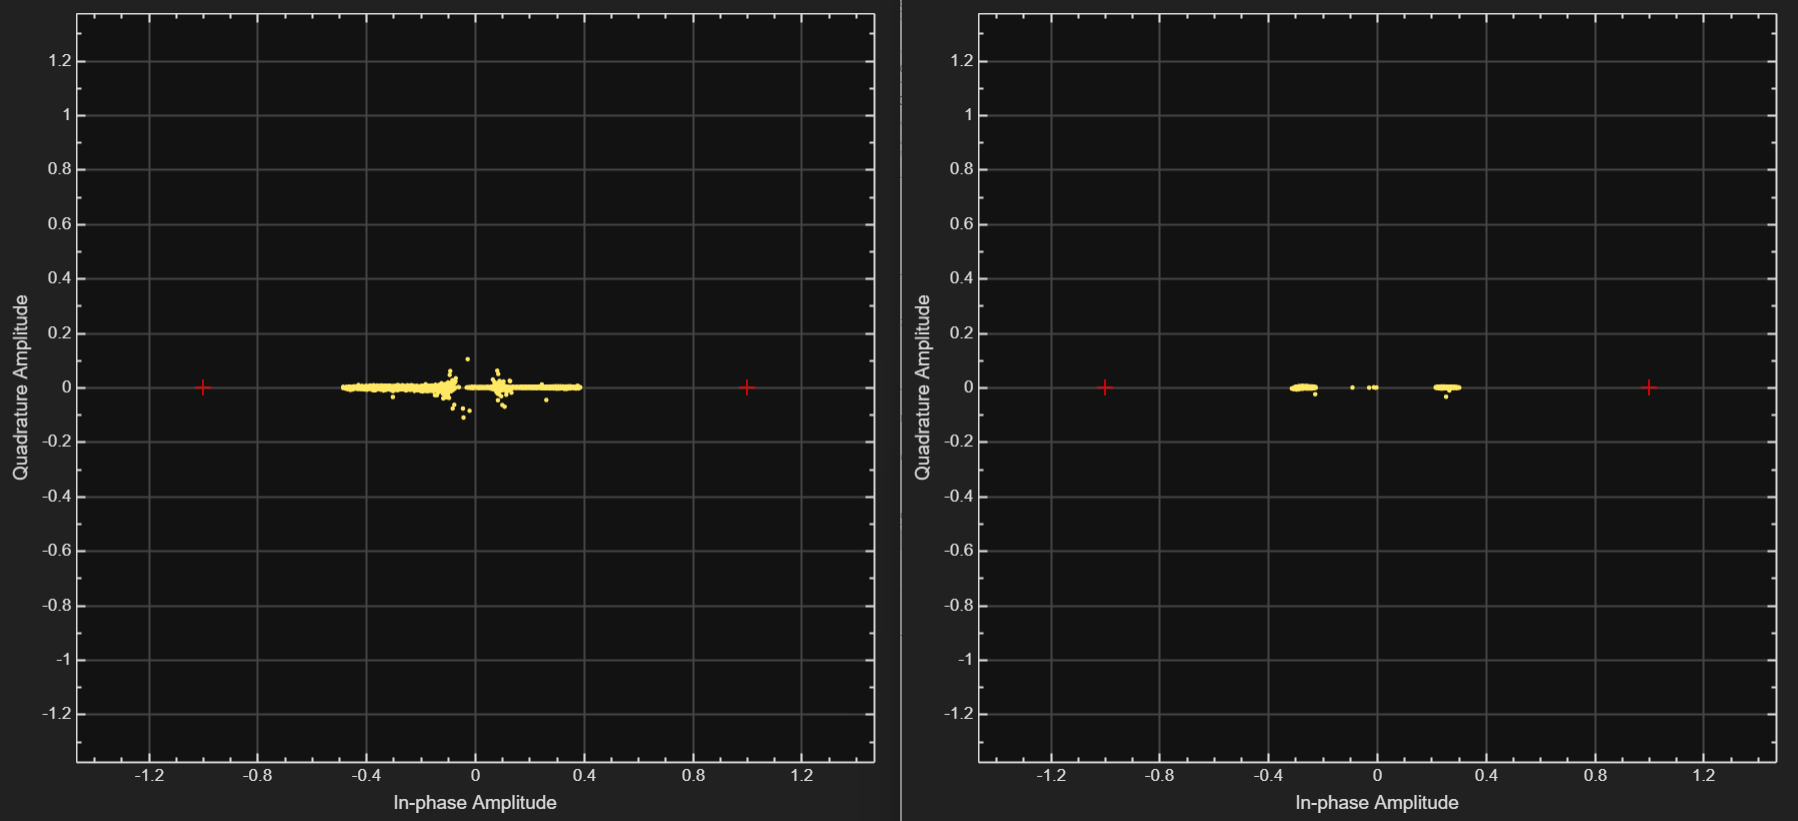
\includegraphics[width=0.7\textwidth]{pluto_constellations_dbpsk.png}}}
	\caption{Constellations Collected with PlutoSDR using Differential Demodulation}
	\label{fig::pluto_constellations_dbpsk}
\end{figure}

\noindent Compared to Figure \ref{fig::pluto_constellations_no_comp}, we see that the differential demodulation resolve the phase offsets. Because our frequency offsets are small, the differential demodulation effectively handles them as well. One additional problem, we observe on hardware but not in simulation is the amplitude of our signal being less than 1. For phase demodulation, this has no impact on the BER. However, it can significantly distort our EVM metric. To compensate for this, we scale our receive data, so it has an average power of 1. Our constellations after performing this scaling are shown in Figure \ref{fig::pluto_constellations_dbpsk_amp_comp}.

\begin{figure}[H]
	\centerline{\fbox{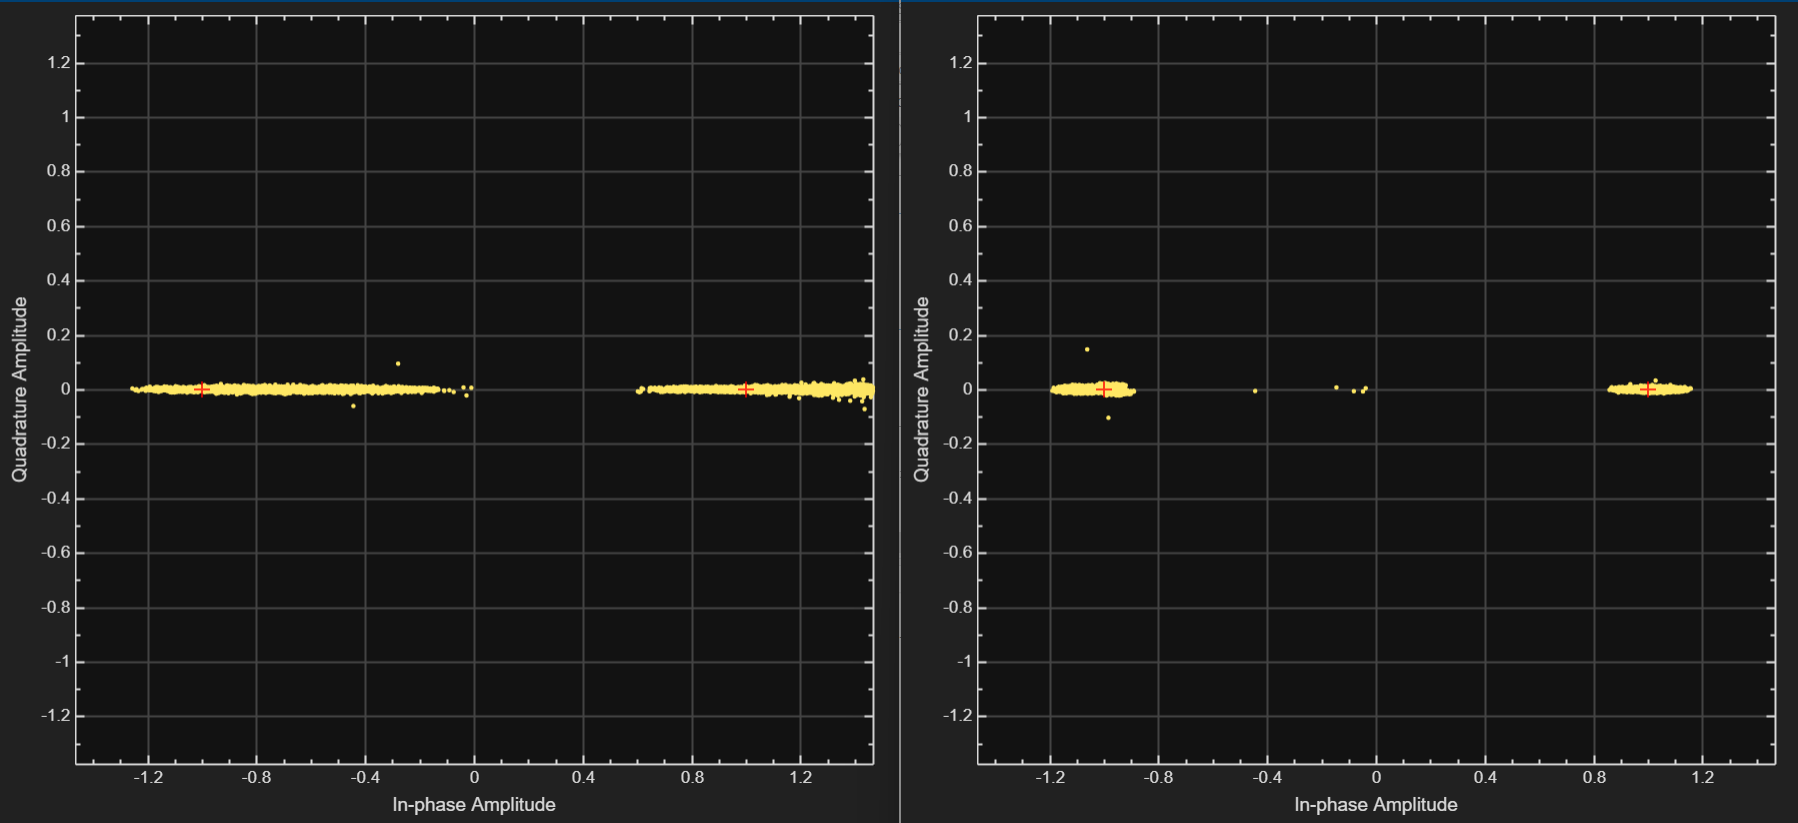
\includegraphics[width=0.7\textwidth]{pluto_constellations_dbpsk_amp_comp.png}}}
	\caption{Constellations Collected with PlutoSDR after Amplitude Correction}
	\label{fig::pluto_constellations_dbpsk_amp_comp}
\end{figure}

\noindent With amplitude correction, differential demodulation, and timing compensation, the constellation looks as we would expect. We can now measure the EVM. To produce results comparable to Sections \ref{section::symbol_timing_compensation} and \ref{section::adding_pieces_together}, we can sweep the PlutoSDR transmitter gain to modify the SNR of the signal. The EVM before timing compensation is shown in Figure \ref{fig::pluto_evm_no_comp} and the EVM after timing compensation is shown in Figure \ref{fig::pluto_evm}.

\begin{figure}[H]
	\centerline{\fbox{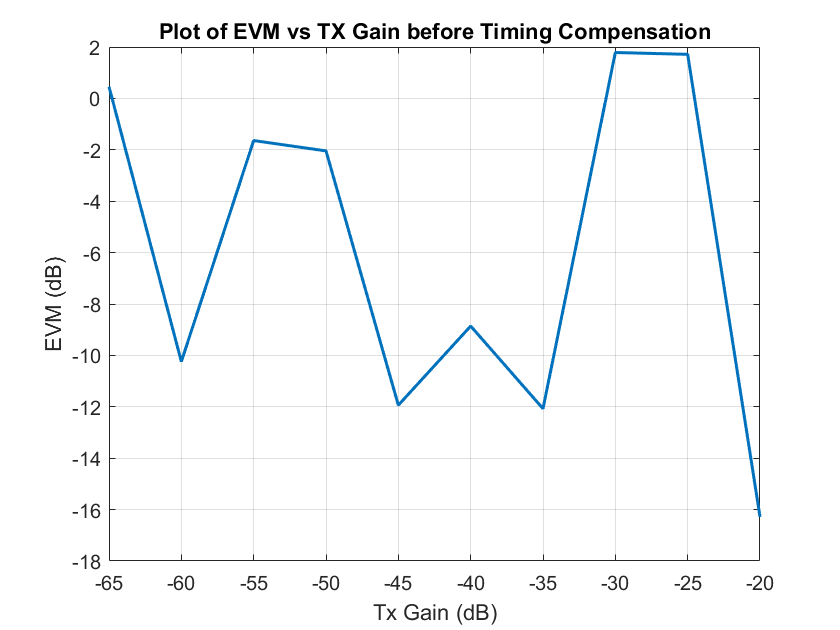
\includegraphics[width=0.5\textwidth]{pluto_evm_no_comp.png}}}
	\caption{Plot of PlutoSDR EVM vs TX Gain before Timing Compensation}
	\label{fig::pluto_evm_no_comp}
\end{figure}

\begin{figure}[H]
	\centerline{\fbox{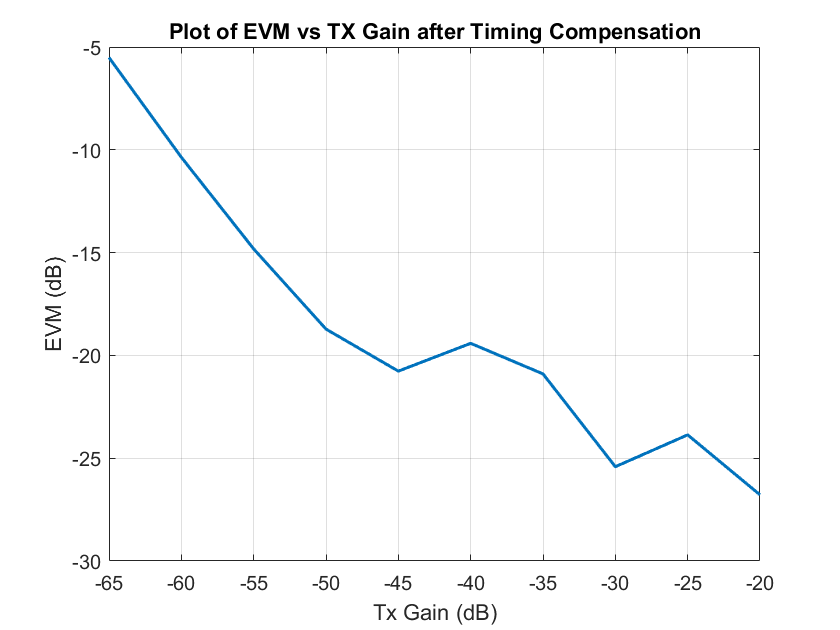
\includegraphics[width=0.5\textwidth]{pluto_evm.png}}}
	\caption{Plot of PlutoSDR EVM vs TX Gain after Timing Compensation}
	\label{fig::pluto_evm}
\end{figure}

\noindent The EVM after timing compensation closely matches the EVM captured in Figure \ref{fig::evm_0p25_symbol_offset}. However, the EVM without timing compensation is very different from the EVM captured in Figure \ref{fig::evm_0p25_symbol_offset_no_comp}. This is because the timing offset varies widely across each of the collected data points. We can visualize this by examining the fractional delay, which is included in Figure \ref{fig::pluto_fractional_delay}.

\begin{figure}[H]
	\centerline{\fbox{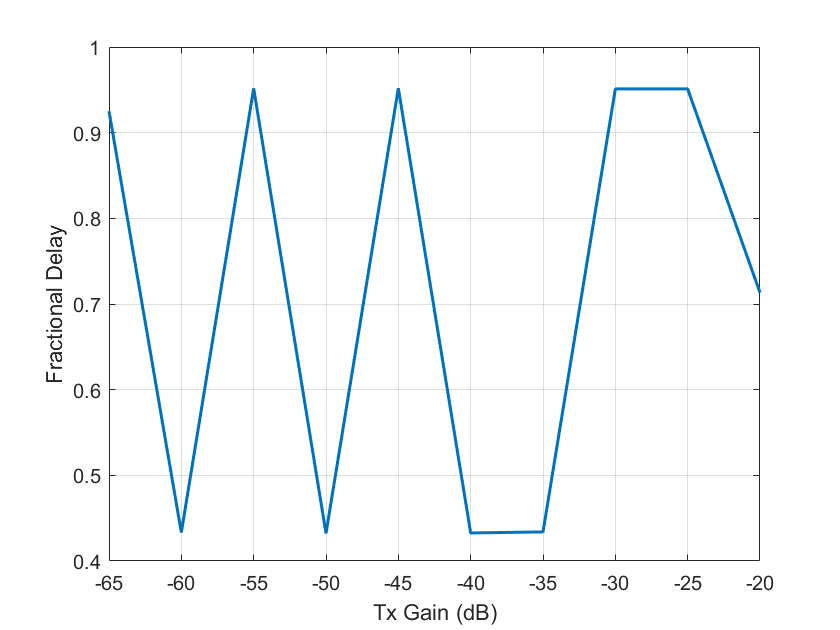
\includegraphics[width=0.5\textwidth]{pluto_fractional_delay.png}}}
	\caption{Plot of Fractional Delay Measured from PlutoSDR Data}
	\label{fig::pluto_fractional_delay}
\end{figure}

\noindent Note that the fractional delays are given at twice the symbol rate. As a result, delays close to 0 or 1 may correspond to a half symbol or full symbol delay, which correspond to the worst and best EVMs respectively.

\section{Conclusion}
% Conclusions to the overall lab that discuss meaningful lessons learned and other takeaways from the assignment. (Important)

In this lab, we learned about pulse shaping, matched filtering, timing errors, and symbol timing synchronization. In regards to pulse shaping and matched filtering, we reviewed the difference between type I and type II Nyquist filters. Both type I and type II Nyquist filters resulted in zero ISI. However, Type I Nyquist filters were defined by a boxcar function in the frequency-domain, while type II Nyquist filters had a more gradual transition. This allowed type II Nyquist filters to have impulse response that decayed faster than the sinc impulse response of a Type I Nyquist filter. This not only made them more practical to implement but also prevented large ISI when there were small timing errors. For this lab, we specifically worked with SRRC filters (a type II Nyquist filter). For this filter, we found that we could maximize the spectral efficiency by decreasing the rolloff factor, $\beta$, and reduce the filter complexity by increasing the rolloff factor. Additionally, we found that large values of $\beta$ improved the performance of timing recovery algorithms due to better defined symbol transitions.

Next, we captured QPSK-modulated data with the PlutoSDR to visualize the impacts of timing error. In this experiment, we saw that timing error increased the spread of our constellation points, resulting in error. We also observed phase offsets, which tilted our constellation. The constellation tilt and phase error persisted even after performing a manual timing compensation.

Then, we learned how to perform timing compensation. Our algorithm for timing compensation included 4 main components: the timing error detector, the loop filter, the interpolation controller, and the interpolator. The timing error detector measured the timing offset. The loop filter stabilized the error correction. The interpolation controller managed the interpolation process, and the interpolator applied a fractional delay to the input samples. To reinforce what we learned, we implemented a custom timing compensation block, which had comparable performance to MATLAB's \texttt{comm.SymbolSychronizer}.

For a slowly varying timing offset, we measured the EVM before and after timing compensation. With timing compensation, we found that the EVM was approximately -SNR at low SNR values. As the SNR increased, we found that the EVM was limited by the drift of the timing offset and imperfections in the system such as the truncated Nyquist impulse response. With a phase offset, we found that the EVM was significantly degraded, and was at best $10\log_{10}(2 - 2\cos\theta)$. In other words, we required phase compensation in addition to timing compensation.

One technique we explored for phase compensation was differential modulation/demodulation, specifically DBPSK. Using this modulation, we were able to achieve similar EVM to our data without a phase shift. However, there was some slight degradation because we used a noisy samples for our differential demodulation.

Our timing compensation logic ran at twice the symbol rate. As a result, when it was integrated into the overall system, it required that the matched filter to output samples at twice the symbol rate. The timing compensation logic also used an "asynchronous FIFO" to pass data between the clock domains. This FIFO received samples on triggers, which occurred once per symbol on average, and outputs samples at the symbol rate.

We also simulated our timing compensation logic under a few other conditions: no timing offset, a static symbol timing offset, and a static phase offset. With no timing offset, we found that our EVM was the same before and after timing synchronization. We also observed the same relationships for timing offsets and phase offsets as our previous experiment.

Finally, we performed timing synchronization using data captured with the PlutoSDR. The data we captured included a phase offset, which we mitigated using DBSPK modulation. We also had to perform amplitude compensation by normalizing our average symbol power to 1. This normalization has no impacts on BER for PSK modulation. However, we needed it to prevent artificial distortion of our EVM. Compared to our simulation results, our EVM with timing compensation was similar. However, our EVM prior to timing compensation was distorted. This occurred because our timing offset was randomized for each point on our EVM curve.

\end{document}